\documentclass[11pt, twoside, pdftex]{article}

% This includes all the settings that we should use for the document
\newcommand{\PDFTitle}{Introduction to the Platform Designer Tool}
\newcommand{\commonPath}{../../Common}
\newcommand{\datePublished}{Mar 2022}

\newcommand{\versnum}{21.1} %version number quartus/AMP
\newcommand{\quartusname}{Quartus\textsuperscript{\textregistered} Prime}	
\newcommand{\textBar}{For \quartusname{} \versnum{}}
\newcommand{\thisyear}{2022 } %for copyright
\newcommand{\company}{FPGAcademy.org}
\newcommand{\longteamname}{FPGAcademy.org}
\newcommand{\teamname}{FPGAcademy}
\newcommand{\website}{FPGAcademy.org}

\newcommand{\productAcronym}{AMP}
\newcommand{\productNameShort}{Monitor Program}

\newcommand{\productNameMedTM}{Monitor Program}
\newcommand{\productNameMed}{Monitor Program}

%\newcommand{\headerLogoFilePath}[1]{#1/FPGAcademy.png}



\setlength\topmargin{-0.25in}
\setlength\headheight{0in}
\setlength\headsep{0.35in}
\setlength\textheight{8.5in}
\setlength\textwidth{7in}
\setlength\oddsidemargin{-0.25in}
\setlength\evensidemargin{-0.25in}
\setlength\parindent{0.25in}
\setlength\parskip{0in} 

\pdfpagewidth 8.5in
\pdfpageheight 11in

% listings is a package that supports encapsulating source code in LaTeX conveniently

\usepackage{listings}
% add support for graphics
\usepackage{graphicx}
\usepackage[usenames, dvipsnames]{color}

\def\expandparam\lstinputlisting[#1]#2{\edef\tmp{\noexpand\lstinputlisting[#1]{#2}}\tmp}

\widowpenalty 10000
\clubpenalty 10000

%%%%%%%%%%%%%%%%%%%% Source Code Formatting %%%%%%%%%%%%%%%%%%%%
\definecolor{globalCommentColour}{rgb}{0.588,0.588,0.588}

%%%%%%%%%%%%%%%%%%%%%%%%%%%%%%%%%%%%%%%%%%%%%%%%%%%%
% Defining a NiosII ASM highlighter for lstlisting
\lstdefinelanguage[NiosII]{Assembler} {
 	morekeywords={add, addi, and, andhi, andi, beq, bge, bgeu, bgt, bgtu, ble,  bleu, blt, bltu, bne, br, break,% 
 	bret, call, callr, cmpeq, cmpeqi, cmpge, cmpgei, cmpgeu, cmpgeui, cmpgt, cmpgti, cmpgtu, cmpgtui, cmple,%
 	cmplei, cmpleu, cmpleui, cmplt, cmplti, cmpltu, cmpltui, cmpne, cmpnei, custom, div, divu, eret, flushd,%
 	flushda, flushi, flushp, initd, initda, initi, jmp, jmpi, ldb, ldbio, ldbu, ldbuio, ldh, ldhio, ldhu, ldhuio,%
 	ldw, ldwio, mov, movhi, movi, movia, movui, mul, muli, mulxss, mulxsu, mulxuu, nextpc, nop, nor, or, orhi, ori,%
 	rdctl, rdprs, ret, rol, roli, ror, sll, slli, sra, srai, srl, srli, stb, stbio, sth, sthio, stw, stwio,%
 	sub, subi, sync, trap, wrctl, wrtcl, wrprs, xor, xori, xorhi, xori},% 	
 	morekeywords=[2]{.abort, .ABORT, .align, .app-file, .ascii, .asciz, .balign, .byte, .comm, .data, .def,%
 	.desc, .dim, .double, .eject, .else, .end, .endef, .endif, .equ, .equiv, .err, .extern, .file, .fill, .float,%
 	.global, .globl, .hword, .ident, .if, .include, .int, .irp, .irpc, .lcomm, .lflags, .line, .linkonce, .ln,%
 	.list, .long, .macro, .mri, .nolist, .octa, .org, .p2align, .psize, .quad, .rept, .sbttl, .scl, .section,%
 	.set, .short, .single, .size, .sleb128, .skip, .space, .stadb, .stabn, .stabs, .string, .symver, .tag,%
 	.text, .title, .type, .val, .uleb128, .word},% 	
 	morekeywords=[3]{et, bt, gp, sp, fp, ea, sstatus, ra, pc, status, estatus, bstatus, ienable, ipending, cpuid,%
 	exception, pteaddr, tlbacc, tlbmisc, eccinj, badaddr, config, mpubase, mpuacc},% 	
 	sensitive=t,%
 	alsoletter=.,%
	morestring=[b]",%
 	morecomment=[s]{/*}{*/},%
 	morecomment=[l]\#,%
   }[keywords,comments,strings]
   
   %% NOTE: morekeywords=[2] are GNU directives.
   
   \definecolor{niosInstructionColour}{rgb}{0.000,0.608,0.000}
   \definecolor{niosDirectiveColour}{rgb}{0.000,0.000,0.902}
   \definecolor{niosSpecialRegColour}{rgb}{0.000,0.000,0.000}
   \definecolor{niosStringColour}{rgb}{0.808,0.482,0.000}
   
   %% NOTE: To make bold use: =\bfseries\color{<colour>}
   \lstdefinestyle{defaultNiosStyle} {
   language=[NiosII]{Assembler},
   stringstyle=\color{niosStringColour},
   keywordstyle=\color{niosInstructionColour},
   keywordstyle=[2]\color{niosDirectiveColour},
   keywordstyle=[3]\itshape\color{niosSpecialRegColour}
   }
%%%%%%%%%%%%%%%%%%%%%%%%%%%%%%%%%%%%%%%%%%%%%%%%%%%%

%%%%%%%%%%%%%%%%%%%%%%%%%%%%%%%%%%%%%%%%%%%%%%%%%%%%
% Defining a ArmA9 ASM highlighter for lstlisting
\lstdefinelanguage[ArmA9]{Assembler} {
 	morekeywords={ADC, ADD, ADDS, AND, ANDS, B, BAL, BEQ, BGE, BGT, BL, BLT, BIC, BKPT, BLX, BNE, BX, CDP, CLZ, CMN, CMP, EOR,%
 	EORS, LDC, LDM, LDR, LDRB, LDRBT, LDRH, LDRSB, LDRSH, LDRT, LSL, MCR, MLA, MOV, MOVW, MOVT, MRC, MRS, MSR, MUL, MVN, ORR, PLD,%
 	ROR, RSB, RSC, SBC, SMLAL, SMULL, STC, STM, STR, STRB, STRBT, STRH, STRT, SUB, SUBS, SWI, SWP, SWPB, TEQ, UMLAL,
 	PUSH, POP, MOVS, RORS, LSR},%
 	morekeywords=[2]{.abort, .ABORT, .align, .app-file, .ascii, .asciz, .balign, .byte, .comm, .data, .def,%
 	.desc, .dim, .double, .eject, .else, .end, .endef, .endif, .equ, .equiv, .err, .extern, .file, .fill, .float,%
 	.global, .globl, .hword, .ident, .if, .include, .int, .irp, .irpc, .lcomm, .lflags, .line, .linkonce, .ln,%
 	.list, .long, .macro, .mri, .nolist, .octa, .org, .p2align, .psize, .quad, .rept, .sbttl, .scl, .section,%
 	.set, .short, .single, .size, .sleb128, .skip, .space, .stadb, .stabn, .stabs, .string, .symver, .tag,%
 	.text, .title, .type, .val, .vectors, .uleb128, .word},%
 	morekeywords=[3]{SP, PC, MIDR, CTR, TCMTR, TLBTR, MPIDR, ID_PFR0, ID_PFR1, ID_DFR0, ID_MMFR0, ID_MMFR1, ID_MMFR2,%
 	ID_MMFR3, ID_ISAR0, ID_ISAR1, ID_ISAR2, ID_ISAR3, ID_ISAR4, CCSIDR, CLIDR, AIDR, CSSELR, TTBR0, TTRB1, TTBR2, DACR,%
 	DFSR, IFSR, ADFSR, AIFSR, DFAAR, IFAR, ICIALLUIS, BPIALLIS, PAR, ICIALLU, ICIMVAU, BPIALL, DCIMVAC, DCISW, V2PCWPR,%
 	DCCVAC, DCCSW, DDIMVAC, DCISW, TLBALLIS, TLBIMVAIS, TLBIASIDIS, TLBIMVAAIS, TLBIALL, TLBIMVA, TLBIASID, TLBIMVAA,%
 	PMCR, PMCNTENSET, PMCNTENCLR, PMOVSR, PMSWINC, PMSELR, PMXEVTYPER, PMXEVCNTR, PMUSERENR, PMINTENSET, PMINTENCLR,%
 	PRRR, NRRR, PLEIDR, PLEASR, PLEFSR, PLEUAR, PLEPCR, VBAR, MVBAR, ISR, FCSEIDR, CONTEXTIDR, TPIDRURW, TPIDRURO, TPIDRPRW},%
 	sensitive=f,%
 	alsoletter=.,%
	morestring=[b]",%
 	morecomment=[s]{/*}{*/},%
 	morecomment=[l]{//},%
   }[keywords,comments,strings]
   
   %% NOTE: morekeywords=[2] are GNU directives.
   
   \definecolor{armInstructionColour}{rgb}{0.000,0.608,0.000}
   \definecolor{armDirectiveColour}{rgb}{0.000,0.000,0.902}
   \definecolor{armSpecialRegColour}{rgb}{0.000,0.000,0.000}
   \definecolor{armStringColour}{rgb}{0.808,0.482,0.000}
   
   \lstdefinestyle{defaultArmStyle} {
   language=[ArmA9]{Assembler},
   stringstyle=\color{armStringColour},
   keywordstyle=\color{armInstructionColour},
   keywordstyle=[2]\color{armDirectiveColour},
   keywordstyle=[3]\itshape\color{armSpecialRegColour}
   }
%%%%%%%%%%%%%%%%%%%%%%%%%%%%%%%%%%%%%%%%%%%%%%%%%%%%

%%%%%%%%%%%%%%%%%%%%%%%%%%%%%%%%%%%%%%%%%%%%%%%%%%%%
% Defining style for the verilog.

\definecolor{verilogCommentColour}{rgb}{0.000,0.502,0.000}

\lstdefinestyle{defaultVerilogStyle} {
language={Verilog},
keywordstyle=\color{blue},
commentstyle=\color{verilogCommentColour}
}
%%%%%%%%%%%%%%%%%%%%%%%%%%%%%%%%%%%%%%%%%%%%%%%%%%%%

%%%%%%%%%%%%%%%%%%%%%%%%%%%%%%%%%%%%%%%%%%%%%%%%%%%%
% Defining style for the vhdl.
\lstdefinestyle{defaultVHDLStyle} {
language={VHDL},
keywordstyle=\color{blue},
commentstyle=\color{verilogCommentColour}
}
%%%%%%%%%%%%%%%%%%%%%%%%%%%%%%%%%%%%%%%%%%%%%%%%%%%%

%%%%%%%%%%%%%%%%%%%%%%%%%%%%%%%%%%%%%%%%%%%%%%%%%%%%
% Java
\definecolor{javaStringColour}{rgb}{0.808,0.482,0}
%%%%%%%%%%%%%%%%%%%%%%%%%%%%%%%%%%%%%%%%%%%%%%%%%%%%

%%%%%%%%%%%%%%%%%%%%%%%%%%%%%%%%%%%%%%%%%%%%%%%%%%%%
% Defining language styles
% C
\definecolor{CStringColour}{rgb}{0.808,0.482,0}
%%%%%%%%%%%%%%%%%%%%%%%%%%%%%%%%%%%%%%%%%%%%%%%%%%%%

%%%%%%%%%%%%%%%%%%%%%%%%%%%%%%%%%%%%%%%%%%%%%%%%%%%%
% Defining extended LaTeX language.
\lstdefinelanguage[LocalLaTeX]{TeX}[LaTeX]{TeX}%
 	{moretexcs={bf, it, sf, lstset},%
   	}%

\lstdefinestyle{defaultLocalLatexStyle} {
language=[LocalLatex]{TeX},
keywordstyle=\color{blue}\bfseries,
keywordstyle=[2]\color{blue},
keywordstyle=[3]\color{blue}\bfseries
}
%%%%%%%%%%%%%%%%%%%%%%%%%%%%%%%%%%%%%%%%%%%%%%%%%%%%

\lstset{
%language = C,
%language = Verilog,
%basicstyle=\color{black}\rmfamily\ttfamily,
basicstyle=\small\color{black}\ttfamily,
commentstyle=\small\color{globalCommentColour}\itshape\ttfamily,
keywordstyle=\small\color{blue}\bfseries\ttfamily,
showstringspaces=false,
frame=none, %lines % boxed listings
breaklines=true,
breakatwhitespace=true,
tabsize=4
}
%%%%%%%%%%%%%%%%%%%%%%%%%%%%%%%%%%%%%%%%%%%%%%%%%%%%%%%%%%%%%%%%


%\usepackage[centering]{geometry}.
%%%%%%%%%%%%%%%%%%%%%%%%%%%%%%%%%%%%%%%%%%%%%%%%%%%
% Document Settings
\usepackage[labelsep=period]{caption}
% we can choose a better font later
%\usepackage{palatino}
\usepackage{fourier}
%\fontencoding{T1}
% include common used symbols
\usepackage{textcomp}
% add support for graphics
\usepackage{graphicx}
\usepackage[usenames, dvipsnames]{color}
% enable to draw thick or thin table hlines
\setlength{\doublerulesep}{\arrayrulewidth}
\usepackage{longtable}
\setlongtables
%\usepackage{array}
% It may be better to use PDFLaTeX as it can generate bookmarks for the
% document

% Add some useful packages
\usepackage{ae,aecompl}
\usepackage{epsfig,float,times}

% reset the font for section
\usepackage{sectsty}
%\allsectionsfont{\fontfamily{ptm}\selectfont}
\allsectionsfont{\usefont{OT1}{phv}{bc}{n}\selectfont}

% use compact space for sections
\usepackage[compact]{titlesec}
\titlespacing{\section}{0pt}{0.2in}{*0}
\titlespacing{\subsection}{0pt}{0.1in}{*0}
\titlespacing{\subsubsection}{0pt}{0.05in}{*0}

% fancyhdr header and footer customization
\usepackage{layout}
\usepackage{fancyhdr}
\pagestyle{fancy}
\fancyhead{}
\fancyhead[R]{\textit{\tiny{\textBar}}}
\fancyfoot{}
\fancyfoot[LO,
RE]{\textrm{\href{https://www.fpgacademy.org}{\small \longteamname}} \\ {\small \datePublished }}
\fancyfoot[RO, LE]{\small \thepage}
% two-side settings
%\fancyhead{} % clear all header fields
%\fancyfoot{} % clear all footer fields
%\fancyfoot[LE,RO]{\thepage}
\renewcommand{\headrulewidth}{2pt}
\renewcommand{\headrule}{{\color{blue} \hrule width\headwidth height\headrulewidth \vskip-\headrulewidth}}
\renewcommand{\footrulewidth}{0pt}

% Format the footer on page 1
\fancypagestyle{plain}{
\fancyhead{}
\fancyfoot{}
\fancyfoot[LO,
RE]{\textrm{\href{https://www.fpgacademy.org}{\small \longteamname}} \\ {\small \datePublished }}
\fancyfoot[RO, LE]{\small \thepage}
\renewcommand{\headrulewidth}{0pt}
}
% adjust some setting to try to make the figure stay in the same page with text
% Reference: 	http://www.cs.uu.nl/~piet/floats/node1.html
%   			http://mintaka.sdsu.edu/GF/bibliog/latex/floats.html
%   General parameters, for ALL pages:
\renewcommand{\topfraction}{0.9}	% max fraction of floats at top
\renewcommand{\bottomfraction}{0.8}	% max fraction of floats at bottom
%   Parameters for TEXT pages (not float pages):
\setcounter{topnumber}{3}
\setcounter{bottomnumber}{3}
\setcounter{totalnumber}{5}     % 2 may work better
\setcounter{dbltopnumber}{2}    % for 2-column pages
\renewcommand{\dbltopfraction}{0.9}	% fit big float above 2-col. text
\renewcommand{\textfraction}{0.07}	% allow minimal text w. figs
%   Parameters for FLOAT pages (not text pages):
\renewcommand{\floatpagefraction}{0.7}	% require fuller float pages
% N.B.: floatpagefraction MUST be less than topfraction !!
\renewcommand{\dblfloatpagefraction}{0.7}	% require fuller float pages
%%%%%%%%%%%%%%%%%%%%%%%%%%%%%%%%%%%%%%%%%%%%%%%%%%%
% remember to use [htp] or [htpb] for placement
%%%%%%%%%%%%%%%%%%%%%%%%%%%%%%%%%%%%%%%%%%%%%%%%%%%

% set no indent for paragraph
\setlength{\parindent}{0em}
\addtolength{\parskip}{11pt}
\newcommand{\compact}{[topsep=0pt]}
% use this package to reduce space
\usepackage{enumitem}
\usepackage{multirow}
\usepackage{rotating}
\usepackage{pifont}
\usepackage{dingbat}
\newcommand{\itemsecond}{$\circ$}
%
%%%%%%%%%%%%%%%%%%
\date{}
\author{}
%%%%%%%%%%%%%%%%%%
\newcommand{\de}{DE-series}
\newcommand{\up}{FPGAcademy}
\newcommand{\fabric}{Avalon Switch Fabric}
\newcommand{\TODO}[1]{\textcolor{red}{\textbf{TODO}: #1}}
\def\registered{{\ooalign{\hfil\raise .00ex\hbox{\scriptsize R}\hfil\crcr\mathhexbox20D}}}

% enable url and reference(bookmarks) in pdf
\usepackage{url}
\usepackage[pdftex, colorlinks]{hyperref}
\hypersetup{%
pdftitle={\PDFTitle},
linkcolor=blue,
hyperindex=true,
pdfauthor={\longteamname},
pdfkeywords={FPGAcademy, Academic Program, Example System},
bookmarksnumbered,
bookmarksopen=false,
filecolor=blue,
pdfstartview={FitH},
urlcolor=blue,
plainpages=false,
pdfpagelabels=true,
linkbordercolor={1 1 1} %no color for link border
}%
%%%%%%%%%%%%%%%%%%%%%%%%%%%%%%%%%%%%%%%%%%%%%%%%%%%
\setlength{\fboxsep}{0.7pt}
\setlength{\fboxrule}{0.5pt}

\newcommand{\red}[1]{{\color{red}\sf{#1}}}
\newcommand{\blue}[1]{{\color{blue}\sf{#1}}}



%%%%%%%%%%%%%%%%%%%%%%%%%
% Add title
\newcommand{\doctitle}{Introduction to the \\ Platform Designer Tool}
\newcommand{\dochead}{Introduction to the Platform Designer Tool}
% Usually no need to change these two lines
\title{\fontfamily{phv}\selectfont{\doctitle} }
\chead{ \small{\textsc{\bfseries \dochead} } }
% Customizations
%%%%%%%%%%%%%%%%%%%%%%%%%
% Allows multiple figures per page

\renewcommand\floatpagefraction{.9}
\renewcommand\topfraction{.9}
\renewcommand\bottomfraction{.9}
\renewcommand\textfraction{.1}   
\setcounter{totalnumber}{50}
\setcounter{topnumber}{50}
\setcounter{bottomnumber}{50}
\raggedbottom

%%%%%%%%%%%%%%%%%%
%%% DOCUMENT START
%\begin{document}
\begin{document}
\begin{table}
    \centering
    \begin{tabular}{p{5cm}p{4cm}}
        \hspace{-3cm}
        &
        \raisebox{1\height}{\parbox[h]{0.5\textwidth}{\Large\fontfamily{phv}\selectfont{\textsf{\doctitle}}}}
    \end{tabular}
    \label{tab:logo}
\end{table}

\colorbox[rgb]{0,0.384,0.816}{\parbox[h]{\textwidth}{\color{white}\textsf{\textit{\textBar}}}}

\thispagestyle{plain}
 
\section{Introduction}

This tutorial presents an introduction to the Intel\textsuperscript{\textregistered} Platform Designer tool, which is
used to design digital hardware systems that contain components such as processors, memories, input/output
interfaces, timers, and the like. The Platform Designer tool allows a designer to choose the components
that are desired in the system by selecting these components in a graphical user interface.
It then automatically generates the hardware system that connects all of the components together.

The hardware system development flow is illustrated by giving step-by-step instructions for using the 
Platform Designer tool in conjunction with the Quartus\textsuperscript{\textregistered} Prime software 
to implement a simple example system. 
The last step in the development process involves configuring the designed hardware system
in an actual FPGA device, and running an application program. To show how this is done, 
it is assumed that the user has access to an Intel DE-series Development and Education board 
connected to a computer that has Quartus Prime and Nios\textsuperscript{\textregistered}
II software installed. The screen captures in the tutorial were obtained using the 
Quartus Prime version \versnum; other versions of the software may be slightly different.

{\bf Contents}:
\begin{itemize}
\item Nios II System
\item Intel's Platform Designer Tool
\item Integration of a Nios II System into a Quartus Prime Project
\item Compiling a Quartus Prime Project when using the Platform Designer Tool
\item Using the \productNameMed{} to Download a Designed Hardware System and Run an Application Program
\end{itemize}
\clearpage
\newpage

\section{Intel DE-series FPGA Boards}
For this tutorial we assume that the reader has access to an Intel DE-series board,
such as the one shown in Figure~\ref{fig:1}. The figure depicts the DE1-SoC board, which features an Intel 
Cyclone\textsuperscript{\textregistered} V FPGA chip. The board provides a lot of other resources, such as memory chips, slider switches,
pushbutton keys, LEDs, audio input/output, video input (NTSC/PAL decoder) and video output (VGA).
It also provides several types of serial input/output connections, including a USB port for
connecting the board to a personal computer. In this tutorial we will make use of only a few of 
the resources: the FPGA chip, slider switches, LEDs, and the USB port that connects to a computer.

Although we have chosen the DE1-SoC board as an example, the tutorial is pertinent for other
DE-series boards that are described in the University Program section of Intel's website. 

\begin{figure}[H]
   \begin{center}
      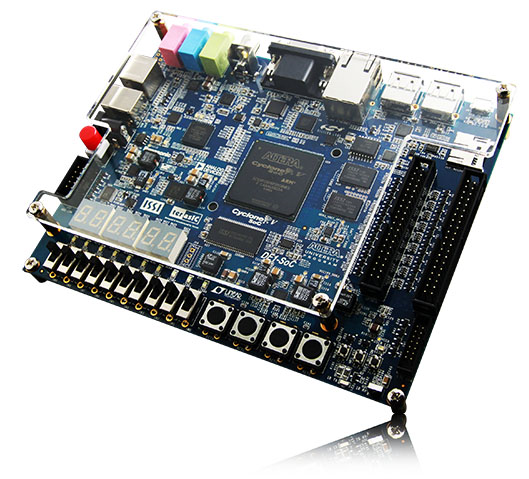
\includegraphics[scale=.5]{figures/figure1.png}
   \end{center}
   \caption{An Intel DE1-SoC board.} 
	\label{fig:1}
\end{figure}

\section{A Digital Hardware System Example}
We will use a simple hardware system that is shown in Figure~\ref{fig:2}.
It includes the Intel Nios II embedded processor,
which is a {\it soft processor} module defined as code in a hardware-description language.
A Nios II module can be included as part of a larger system, and then that system can
be implemented in an Intel FPGA chip by using the Quartus Prime software.

\begin{figure}[H]
   \begin{center}
      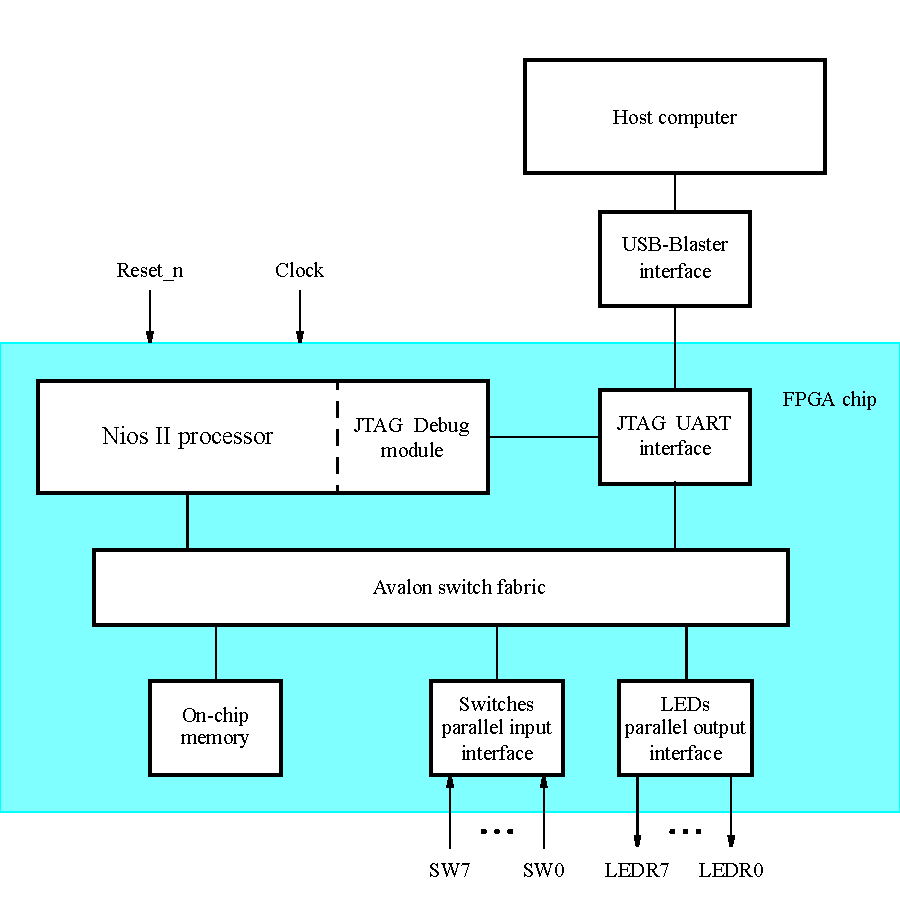
\includegraphics[scale=1]{figures/figure2.pdf}
   \end{center}
   \caption{A simple example of a Nios II system.} 
	\label{fig:2}
\end{figure}

As shown in Figure~\ref{fig:2}, the Nios II processor is connected to the memory and I/O interfaces 
by means of an interconnection network called the {\it Avalon\textsuperscript{\textregistered} switch fabric}.
This interconnection network is automatically generated by the Platform Designer tool.

The memory component in our system will be realized by using the on-chip memory
available in the FPGA chip.
The I/O interfaces that connect to the slider switches and LEDs will be implemented by
using the predefined modules that are available in the Platform Designer tool.
A special JTAG* UART interface is used to connect to the circuitry that provides a USB
link to the host computer to which the DE-series board is connected. This circuitry and the
associated software is called the {\it USB-Blaster}. Another module, called the
JTAG Debug module, is provided to allow the host computer to control the Nios II system.
It makes it possible to perform operations such as downloading Nios II programs into memory,
starting and stopping the execution of these programs, setting breakpoints, and examining the 
contents of memory and Nios II registers.

Since all parts of the Nios II system implemented on the FPGA chip are defined by
using a hardware description language, a knowledgeable user could write such code
to implement any part of the system. This would be an onerous and time consuming
task. Instead, we will show how to use the Platform Designer tool to implement the desired system simply by
choosing the required components and specifying the parameters needed to make
each component fit the overall requirements of the system. Although in this tutorial we
illustrate the capability of the Platform Designer tool by designing a very simple
system, the same approach is used to design larger systems.

Our example system in Figure~\ref{fig:2} is intended to realize a trivial task.
Eight slider switches on the DE1-SoC board, $SW7-0$, are used to turn on
or off eight LEDs, $LEDR7-0$. To achieve the desired operation,
the eight-bit pattern corresponding to the state of the switches has to be 
sent to the output port to activate the LEDs. This will be done
by having the Nios II processor execute a program stored in the on-chip memory.
Continuous operation is required, such that as the switches are toggled the lights
change accordingly. 

In the next section we will use the Platform Designer tool to design the hardware depicted in Figure~\ref{fig:2}.
After assigning the FPGA pins to realize the connections between
the parallel interfaces and the switches and LEDs on the DE1-SoC board,
we will compile the designed system.
Finally, we will use the software tool called the {\it \productNameMed{}} to 
download the designed circuit into the FPGA device, and 
download and execute a Nios II program that performs the desired task.

Doing this tutorial, the reader will learn about:
\begin{itemize}
\item Using the Platform Designer tool to design a Nios II-based system
\item Integrating the designed Nios II system into a Quartus Prime project
\item Implementing the designed system on the DE1-SoC board
\item Running an application program on the Nios II processor
\end{itemize}

\section{Intel's Platform Designer Tool}

The Platform Designer tool is used in conjunction with the Quartus Prime CAD software.
It allows the user to easily create a system based on the Nios II processor, by simply
selecting the desired functional units and specifying their parameters.
To implement the system in Figure~\ref{fig:2}, we have to instantiate the following functional
units:
\begin{itemize}
\item Nios II processor
\item On-chip memory, which consists of the memory blocks in the FPGA chip;
we will specify a 4-Kbyte memory arranged in 32-bit words
\item Two parallel I/O interfaces
\item JTAG UART interface for communication with the host computer
\end{itemize}

\noindent To define the desired system, start the Quartus Prime software and perform
the following steps: 
\begin{enumerate}
\item Create a new Quartus Prime project for your system. As shown in Figure~\ref{fig:3}, we stored 
our project in a directory called {\it platformdesigner\_tutorial}, and we
assigned the name {\it lights} to both the project and its top-level design entity.
You can choose a different directory or project name.
Step through the screen for adding design files to the project;
we will add the required files later in the tutorial.
In your project, choose the FPGA device used on your DE-series board. 
A list of FPGA devices on the DE-series boards is given in Table~\ref{tab:device}. 

\begin{figure}[H]
			\begin{center}
      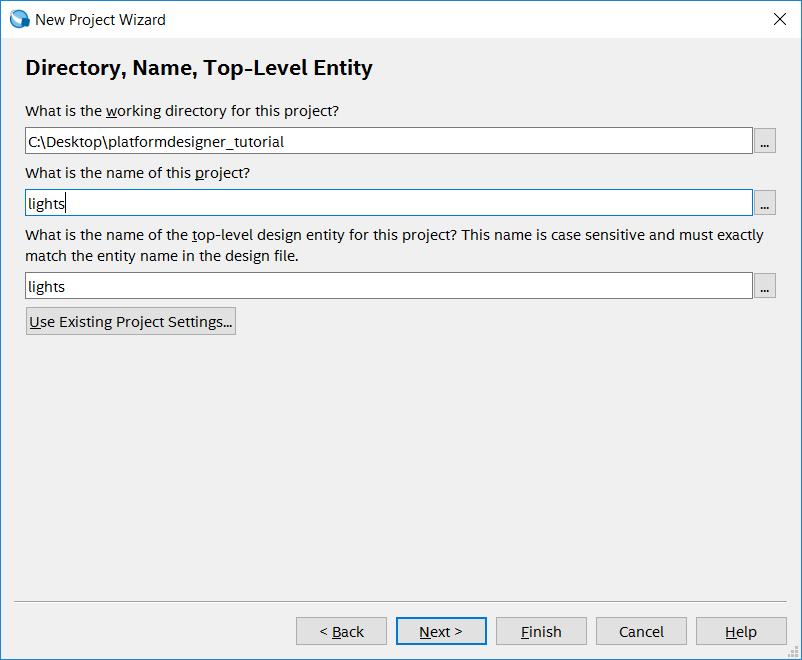
\includegraphics[scale=0.6]{figures/figure3.png}
     	\end{center}
   	\caption{Create a new project.} 
	\label{fig:3}
	\end{figure}

\begin{table}[H]
	\begin{center}
	\begin{tabular}{| c | c |}
	\hline
	Board & Device Name \\
	\hline
	DE0-CV & Cyclone\textsuperscript{\textregistered} V 5CEBA4F23C7 \\
	\hline
	DE0-Nano & Cyclone\textsuperscript{\textregistered} IVE EP4CE22F17C6 \\
	\hline
	DE0-Nano-SoC & Cyclone\textsuperscript{\textregistered} V SoC 5CSEMA4U23C6\\
	\hline
	DE1-SoC & Cyclone\textsuperscript{\textregistered} V SoC 5CSEMA5F31C6 \\
	\hline
	DE2-115 & Cyclone\textsuperscript{\textregistered} IVE EP4CE115F29C7 \\
	\hline
	DE10-Lite & Max\textsuperscript{\textregistered} 10 10M50DAF484C7G \\
	\hline
	DE10-Standard & Cyclone\textsuperscript{\textregistered} V SoC 5CSXFC6D6F31C6 \\
	\hline
	DE10-Nano & Cyclone\textsuperscript{\textregistered} V SE 5CSEBA6U2317 \\
	\hline
	\end{tabular}
	\caption{DE-series FPGA device names}
	\label{tab:device}
	\end{center}
\end{table}

\item After completing the New Project Wizard to create the project,
in the main Quartus Prime window select {\sf Tools $>$ Platform Designer}, which leads to 
the window in Figure~\ref{fig:4}.
This is the System Contents tab of the Platform Designer tool, which is used to
add components to the system and configure the selected components to meet the design
requirements. The available components are listed on the left side of the window.


\begin{figure}[H]
   \begin{center}
      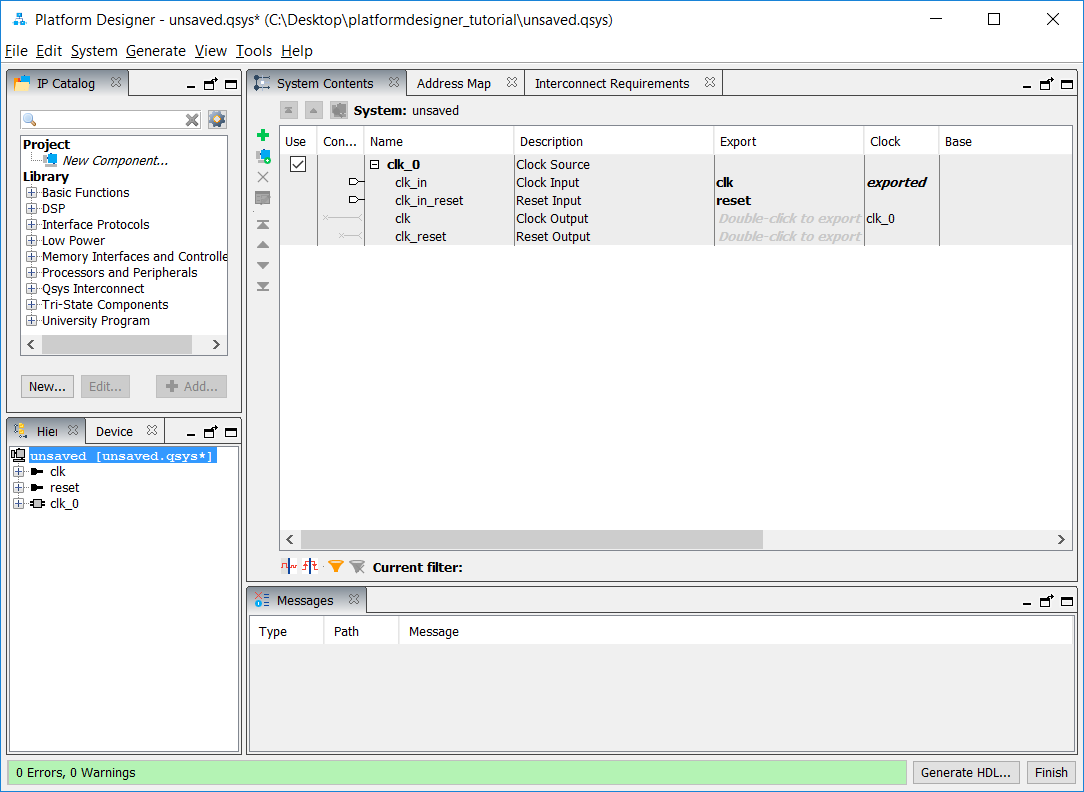
\includegraphics[scale=0.55]{figures/figure4.png}
   \end{center}
   \caption{Create a new Nios II system.} 
	\label{fig:4}
\end{figure}

\item  The hardware system that will be generated using the Platform Designer tool
runs under the control of a clock. For this tutorial we
will make use of the 50-MHz clock that is provided on the DE1-SoC board.
Your hardware system should contain a clock source called {\it clk\_0}, whose
frequency is 50-MHz. You can check that its frequency is indeed 50-MHz by
double clicking the component, and checking the {\sf Clock frequency} parameter of the component.
If your system does not already contain {\it clk\_0}, it is possible to add a clock source by selecting 
{\sf Basic Functions > Clocks; PLLs and Resets > Clock Source} in the {\sf IP Catalog} tab, then clicking {\sf Add...}.
~\\

\item Next, specify the processor as follows:
\begin{itemize}
\item On the left side of the Platform Designer window expand {\sf Processors and Peripherals}, select 
{\sf Embedded Processors > Nios II Processor}
and click {\sf Add...}, which leads to the window in Figure~\ref{fig:6}.

\begin{figure}[H]
   \begin{center}
      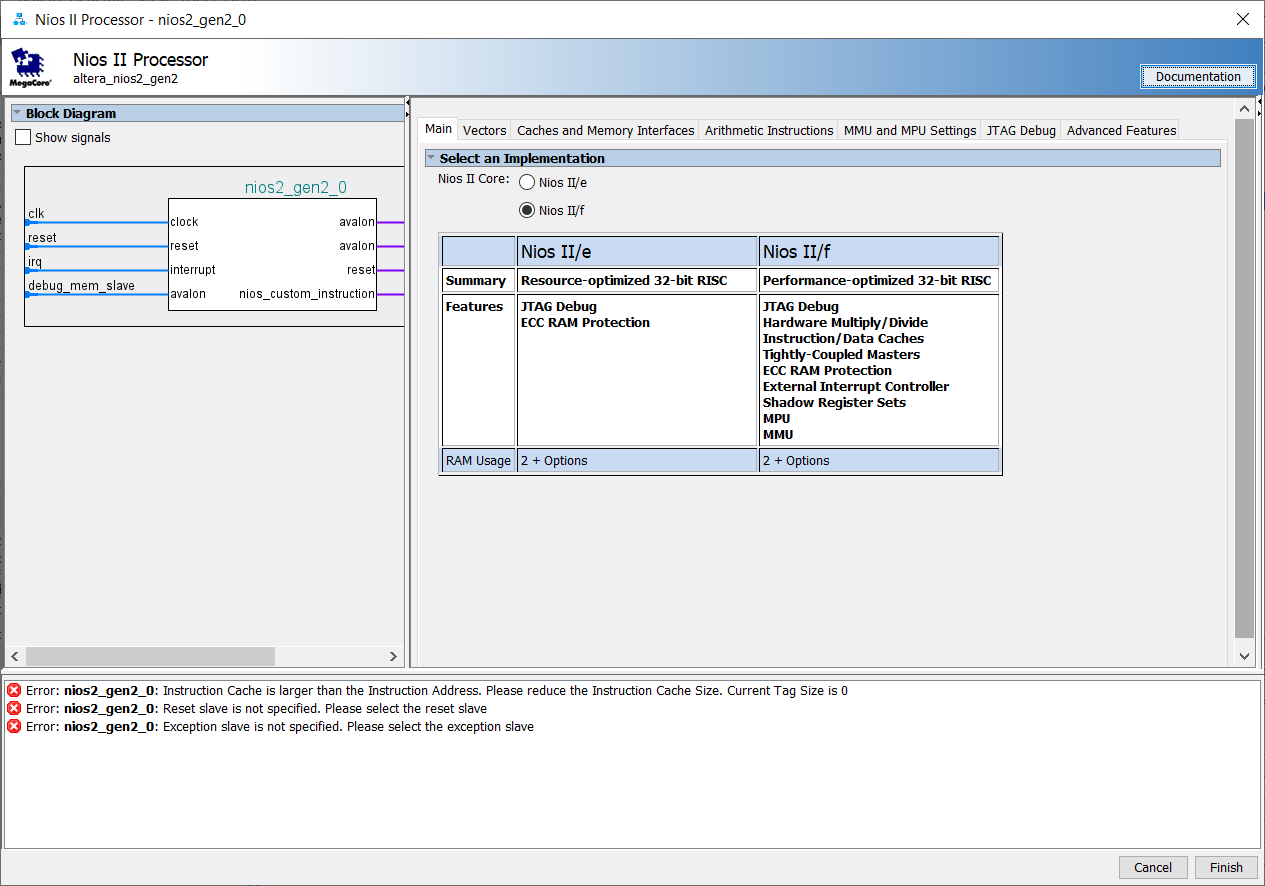
\includegraphics[scale=0.5]{figures/figure6.png}
   		\caption{Create a Nios II processor.} 
			\label{fig:6}
	  \end{center}
\end{figure}
\item Choose Nios II/e which is the economy version of the processor. This version is available for use without a paid license.
The Nios II processor has {\it reset} and
{\it interrupt} inputs. When one of these inputs is activated, the processor starts executing 
the instructions stored at memory addresses known as {\it reset vector} and
{\it interrupt vector}, respectively. Since we have not yet included any memory components in
our design, the Platform Designer tool will display corresponding error messages. Ignore these messages 
as we will provide the necessary information later.
Click {\sf Finish} to return to the main Platform Designer window, which now shows
the Nios II processor specified as indicated in Figure~\ref{fig:7}. 
\end{itemize}

\begin{figure}[H]
   \begin{center}
      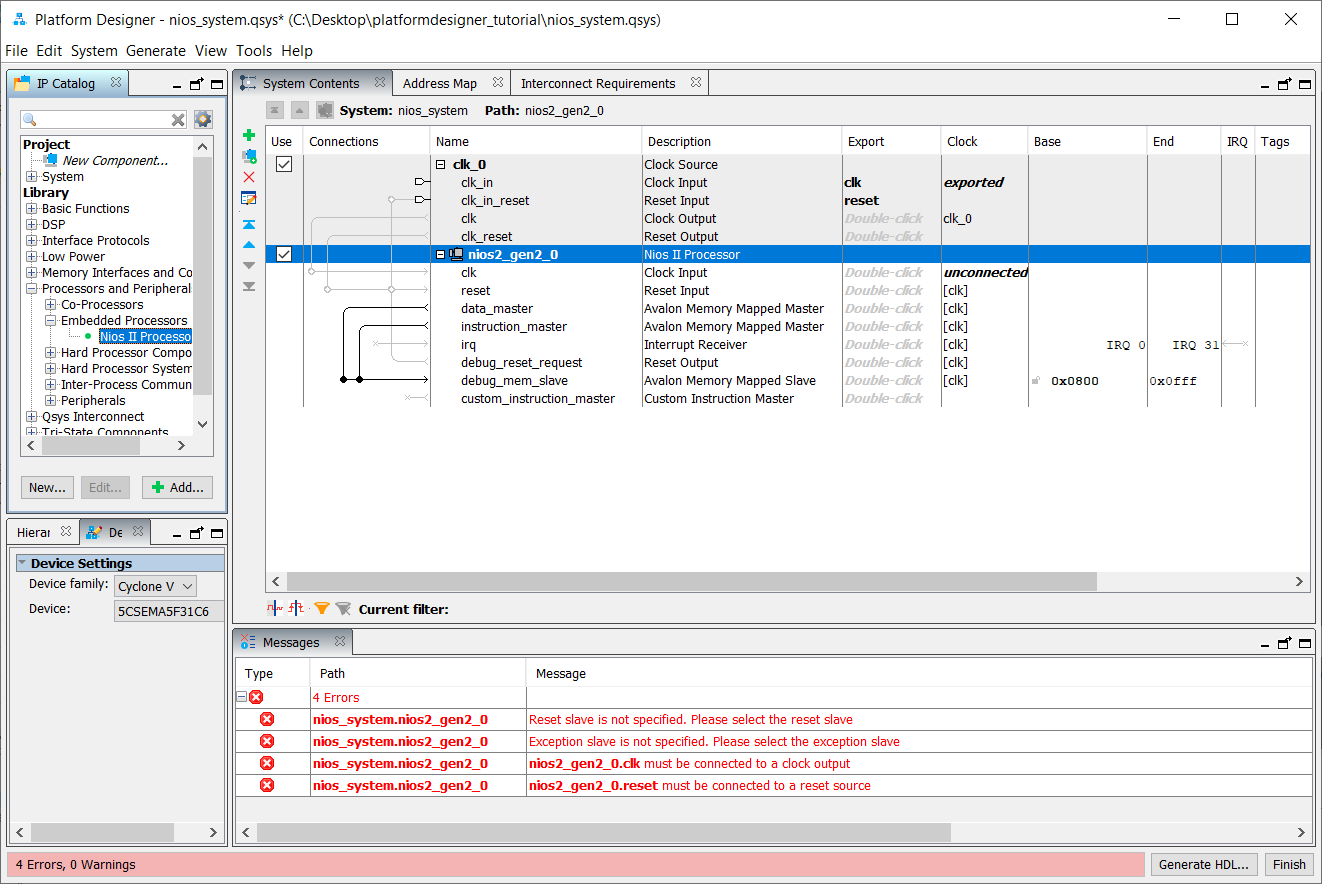
\includegraphics[scale=0.55]{figures/figure7.png}
   \end{center}
   \caption{Inclusion of the Nios II processor in the design.} 
	\label{fig:7}
\end{figure}

\item To specify the on-chip memory perform the following:
\begin{itemize}
\item Expand the category {\sf Basic Functions}, and then expand to select
{\sf On Chip Memory $>$ On-Chip Memory (RAM or ROM) Intel FPGA IP},
and click {\sf Add}
\item In the On-Chip Memory Configuration Wizard window, shown in Figure~\ref{fig:8}, ensure that
the {\sf Slave S1 Data width} is set to 32 bits and the {\sf Total memory size} to 4K bytes (4096 bytes)
\item Do not change the other default settings
\item Click {\sf Finish}, which returns to the System Contents tab as indicated
in Figure~\ref{fig:9}
\end{itemize}

\begin{figure}[H]
   \begin{center}
      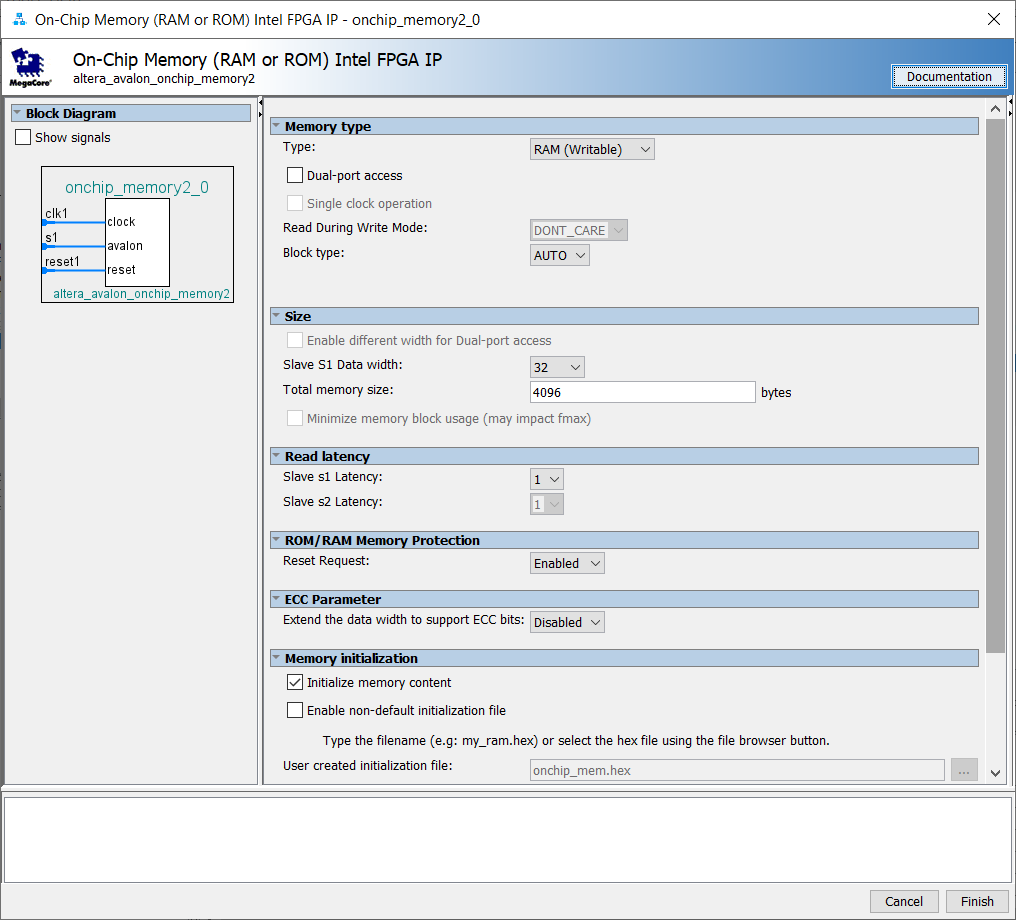
\includegraphics[scale=0.6]{figures/figure8.png}
   \end{center}
   \caption{Define the on-chip memory.} 
	\label{fig:8}
\end{figure}

\item Observe that while the Nios II processor and the on-chip memory have been included
in the design, no connections between these components have been established. To specify the
desired connections, examine the {\sf Connections} area in the window in 
Figure~\ref{fig:9}. The connections already made
are indicated by filled circles and the other possible connections by empty circles,
as indicated in Figure~\ref{fig:10}.

Clicking on an empty circle makes a connection.
Clicking on a filled circle removes the connection.

Make the following connections:
\begin{itemize}
\item Clock inputs of the processor and the memory to the clock output of the clock component
\item Reset inputs of the processor and the memory to both the reset output of the clock component
and the {\it debug\_reset\_request} output
\item The {\it s1} input of the memory to both the {\it data\_master} and {\it instruction\_master}
outputs of the processor
\end{itemize}

The resulting connections are shown in Figure~\ref{fig:11}. 

\begin{figure}[H]
   \begin{center}
      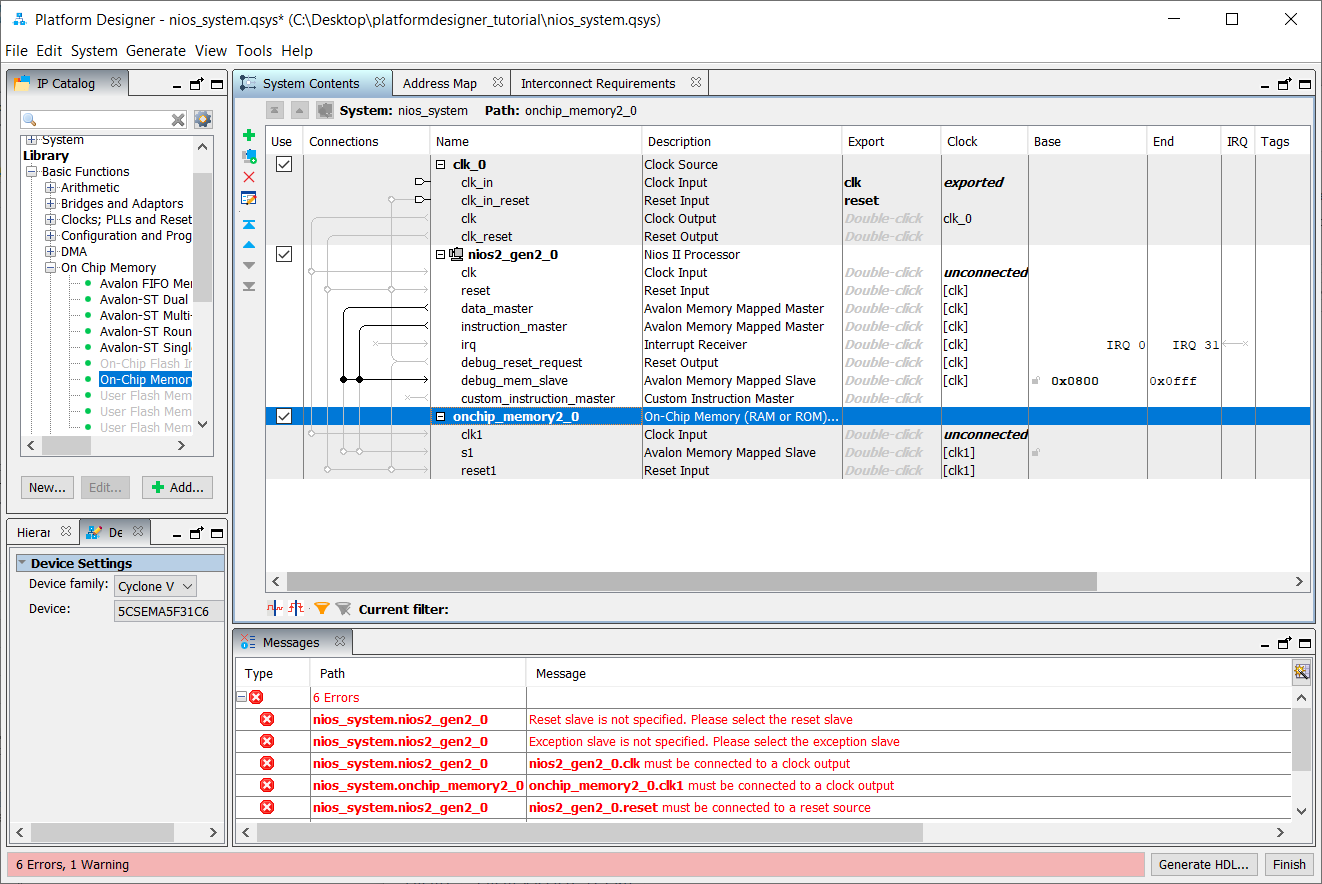
\includegraphics[scale=0.55]{figures/figure9.png}
   \end{center}
   \caption{The on-chip memory included on a DE-series board.} 
	\label{fig:9}
\end{figure}

\begin{figure}[H]
   \begin{center}
      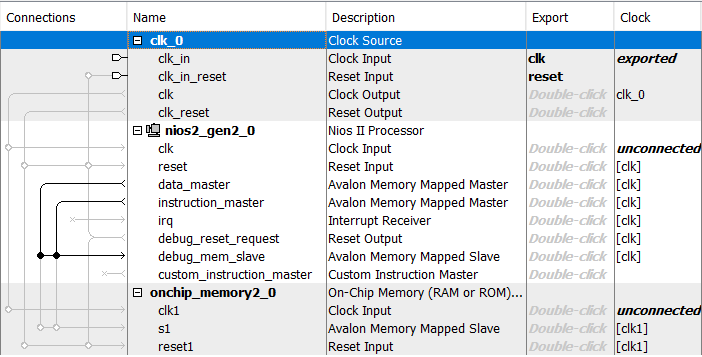
\includegraphics[scale=0.7]{figures/figure10.png}
   \end{center}
   \caption{Connections that can be made.} 
	\label{fig:10}
\end{figure}

\begin{figure}[H]
   \begin{center}
      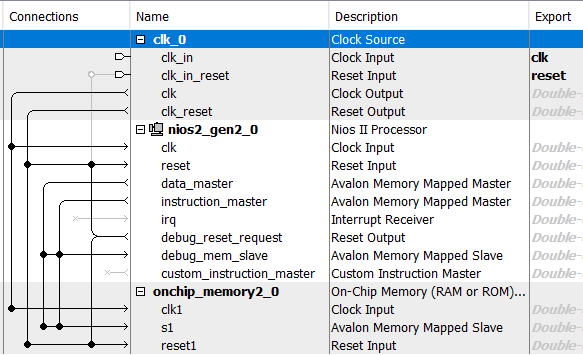
\includegraphics[scale=0.7]{figures/figure11.png}
   \end{center}
   \caption{The connections that are now established.} 
	\label{fig:11}
\end{figure}

\item Specify the input parallel I/O interface as follows:
\begin{itemize}
\item From the IP Catalog, select {\sf Processors and Peripherals $>$ Peripherals $>$ PIO (Parallel I/O) Intel FPGA IP}
and click {\sf Add} to reach the PIO Configuration Wizard in Figure~\ref{fig:12}
\item Specify the width of the port to be 8 bits and choose the direction of the 
port to be {\sf Input}, as shown in the figure. 
\item Click {\sf Finish}. 
\end{itemize}

\begin{figure}[H]
   \begin{center}
      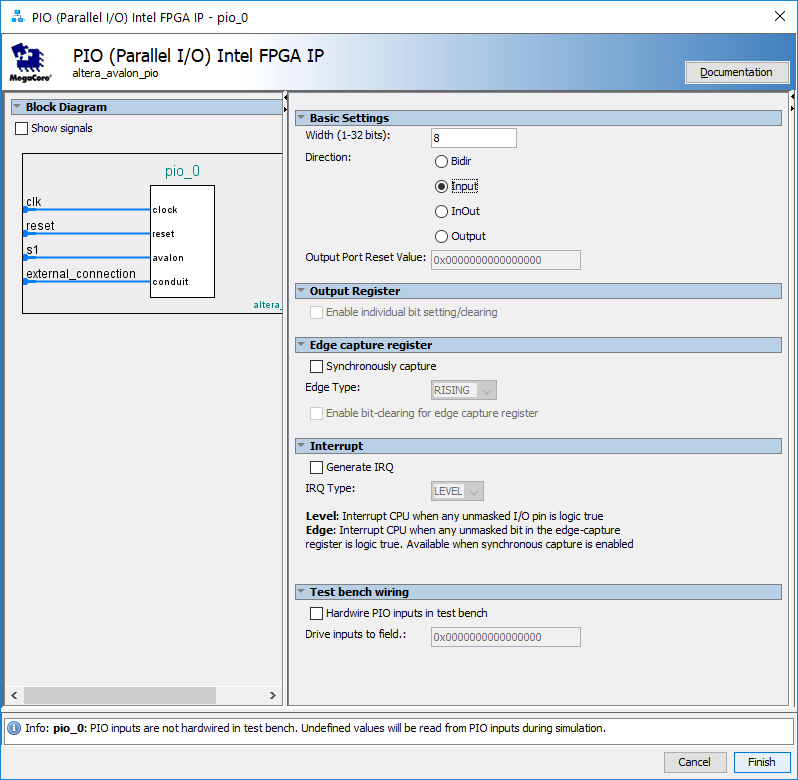
\includegraphics[scale=0.6]{figures/figure12.png}
   \end{center}
   \caption{Define a parallel input interface.} 
	\label{fig:12}
\end{figure}

\item In the same way, specify the output parallel I/O interface: 
\begin{itemize}
\item From the IP Catalog, select {\sf Processors and Peripherals $>$ Peripherals $>$ PIO (Parallel I/O) Intel FPGA IP}
and click {\sf Add} to reach the PIO Configuration Wizard again
\item Specify the width of the port to be 8 bits and choose the direction of the 
port to be {\sf Output}. 
\item Click {\sf Finish} to return to the System Contents tab
\end{itemize}

\item Specify the necessary connections for the two PIOs:
\begin{itemize}
\item Clock input of the PIO to the clock output of the clock component
\item Reset input of the PIO to the reset output of the clock component
and the {\it debug\_reset\_request} output
\item The {\it s1} input of the PIO the {\it data\_master} output of the processor
\end{itemize}
The resulting design is depicted in Figure~\ref{fig:13}.

\begin{figure}[H]
   \begin{center}
      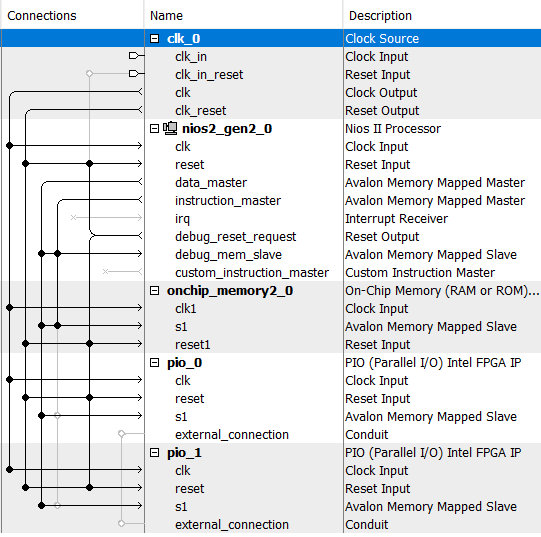
\includegraphics[scale=0.7]{figures/figure13.png}
   \end{center}
   \caption{The system with all components and connections.} 
	\label{fig:13}
\end{figure}

\item We wish to connect to a host computer and provide a means for communication
between the Nios II system and the host computer. This can be accomplished by 
instantiating the JTAG UART interface as follows:
\begin{itemize}
\item Select {\sf Interface Protocols $>$ Serial $>$ JTAG UART Intel FPGA IP} and
click {\sf Add} to reach the JTAG UART Configuration Wizard in Figure~\ref{fig:14}
\item Do not change the default settings 
\item Click {\sf Finish} to return to the System Contents tab
\end{itemize}
Connect the JTAG UART to the clock, reset and data-master ports, as was done for the PIOs. Connect the Interrupt Request (IRQ) line from the JTAG UART to the Nios II processor by selecting the connection under the IRQ column, as shown in Figure~\ref{fig:15}. Once the connection is made, a box with the number 0 inside will appear on the connection. The Nios II processor has 32 interrupt ports ranging from 0 to 31, and the number in this box selects which port will be used for this IRQ. Click on the box and change it to use port 5. Make sure the {\it irq} port of JTAG UART gets automatically connected to the {\it irq} port of Nios II Processor.

\begin{figure}[H]
   \begin{center}
      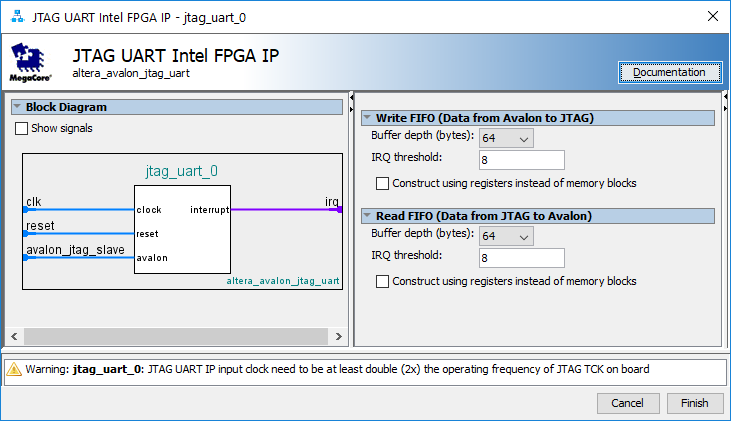
\includegraphics[scale=0.55]{figures/figure14.png}
   \end{center}
   \caption{Define the JTAG UART interface.} 
	\label{fig:14}
\end{figure}

\begin{figure}[H]
   \begin{center}
      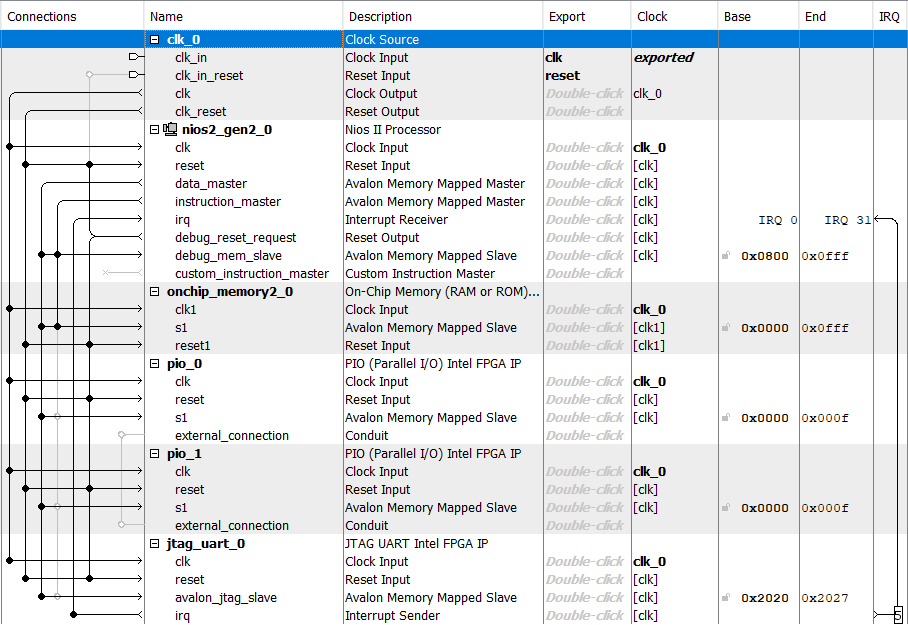
\includegraphics[scale=0.65]{figures/figure15.png}
   \end{center}
   \caption{Connect the IRQ line from the JTAG UART to the Nios II processor.} 
	\label{fig:15}
\end{figure}


\item Note that the Platform Designer tool automatically chooses names for the various components. The names are not
necessarily descriptive enough to be easily associated with the target design, 
but they can be changed.
In Figure~\ref{fig:2}, we use the names Switches and LEDs for the parallel input and output
interfaces, respectively. These names can be used in the implemented system.
Right-click on the {\sf pio\_0} name and then select {\sf Rename}. Change the
name to {\it switches}. Similarly, change {\sf pio\_1} to {\it LEDs}.
Figure~\ref{fig:16} shows the system with name changes that we made for all components.

\begin{figure}[H]
   \begin{center}
      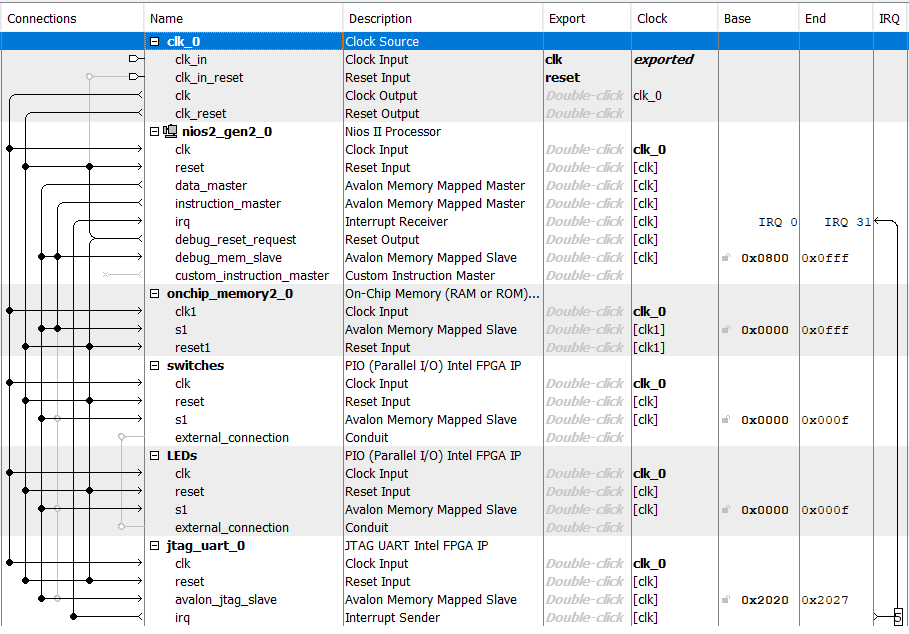
\includegraphics[scale=0.7]{figures/figure16.png}
   \end{center}
   \caption{The system with all components appropriately named.} 
	\label{fig:16}
\end{figure}

\item Observe that the base and end addresses of the various components in the designed system
have not been properly assigned. These addresses can be assigned by the user, 
but they can also be assigned automatically by the Platform Designer tool. We will choose the latter possibility.
However, we want to make sure that the on-chip memory has the base address of zero. 
Double-click on the Base address for the on-chip memory in the Platform Designer window and enter 
the address 0x00000000. Then, lock this address by clicking on the adjacent lock symbol.
Now, let the Platform Designer assign the rest of the addresses by selecting
{\sf System $>$ Assign Base Addresses} (at the top of the window), which produces an
assignment similar to that shown in Figure~\ref{fig:17}.
 

\begin{figure}[H]
   \begin{center}
      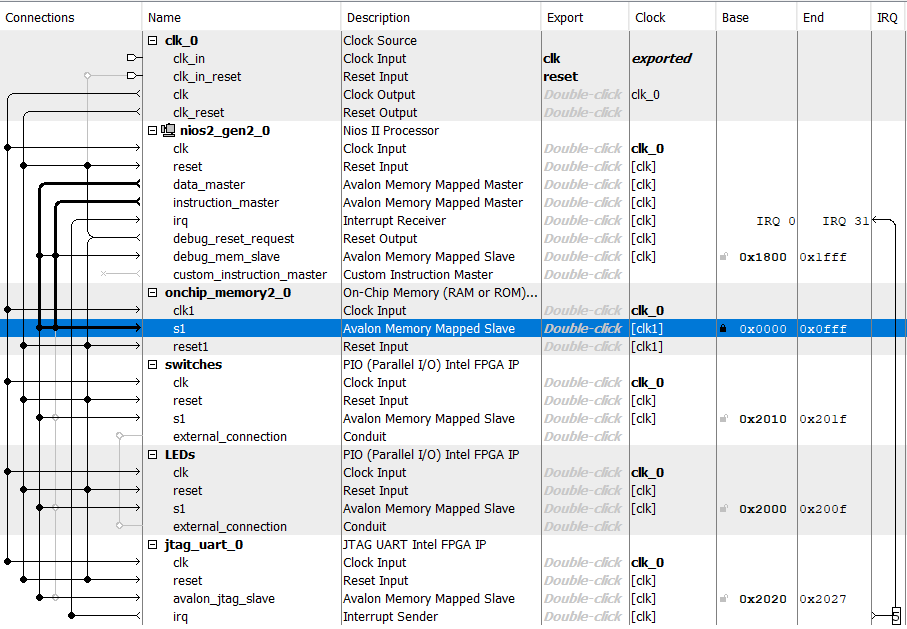
\includegraphics[scale=0.7]{figures/figure17.png}
   \end{center}
   \caption{The system with assigned addresses.} 
	\label{fig:17}
\end{figure}

\item The behavior of the Nios II processor when it is reset is defined by its reset vector. 
It is the location in the memory device from which the processor fetches the next instruction when it is reset. 
Similarly, the exception vector is the memory address of the instruction that the processor 
executes when an interrupt is raised. 
To specify these two parameters, perform the following: 
\begin{itemize}
\item	Right-click on the {\it nios2\_gen2\_0} component (it may be called {\it nios2\_processor} in some versions of the Platform Designer) in the window displayed in 
Figure~\ref{fig:17}, and then select {\sf Edit} to reach the window in Figure~\ref{fig:18}
\item	Select {\it onchip\_memory2\_0.s1} to be the memory device for both reset 
and exception vectors, as shown in Figure~\ref{fig:18}
\item	Do not change the default settings for offsets
\item Observe that the error messages dealing with memory assignments shown in 
Figure~\ref{fig:6} will now disappear 
\item	Click {\sf Finish} to return to the System Contents tab
\end{itemize}

\begin{figure}[H]
   \begin{center}
      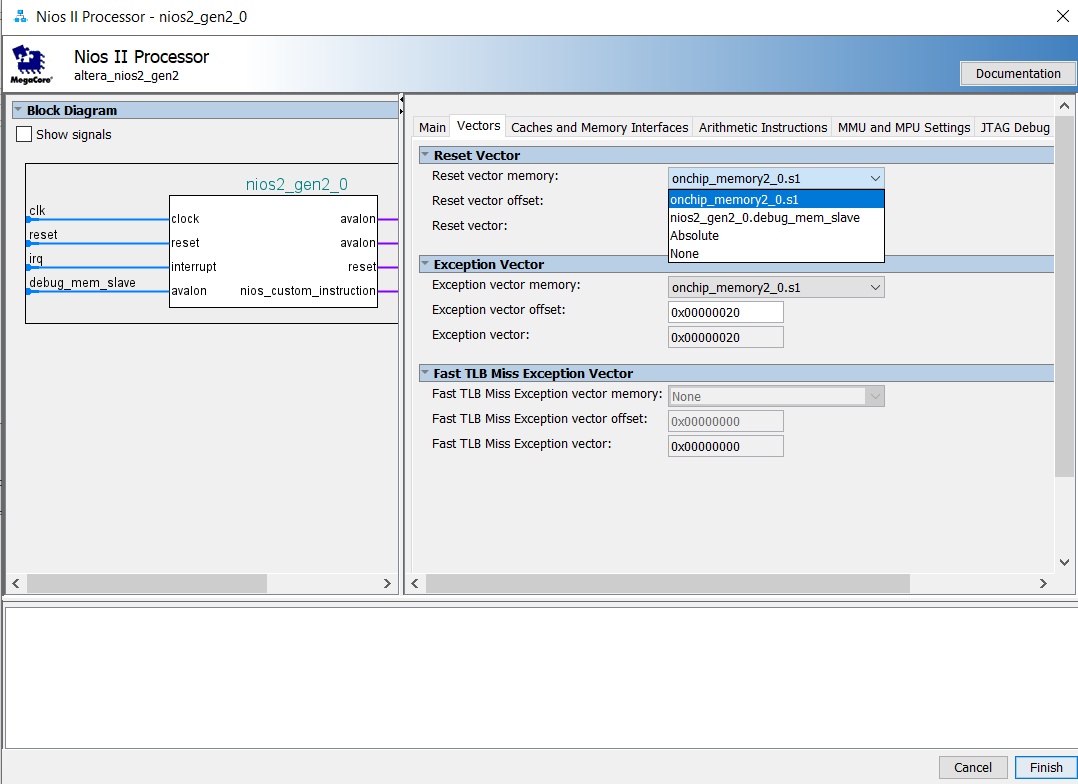
\includegraphics[scale=0.52]{figures/figure18.png}
   \end{center}
   \caption{Define the reset and exception vectors.} 
	\label{fig:18}
\end{figure}

\item So far, we have specified all connections inside our {\it nios\_system} circuit.
It is also necessary to specify connections to external components, which are switches and LEDs
in our case. To accomplish this, double click on {\sf Double-click to export} (in the Export column of the System
Contents tab) for {\sf external\_connection} of the switches PIO, and type the name {\it switches}.
Similarly, establish the external connection for the lights, called {\it leds}.
This completes the specification of our {\it nios\_system}, which is depicted in Figure~\ref{fig:19}.

\begin{figure}[H]
   \begin{center}
      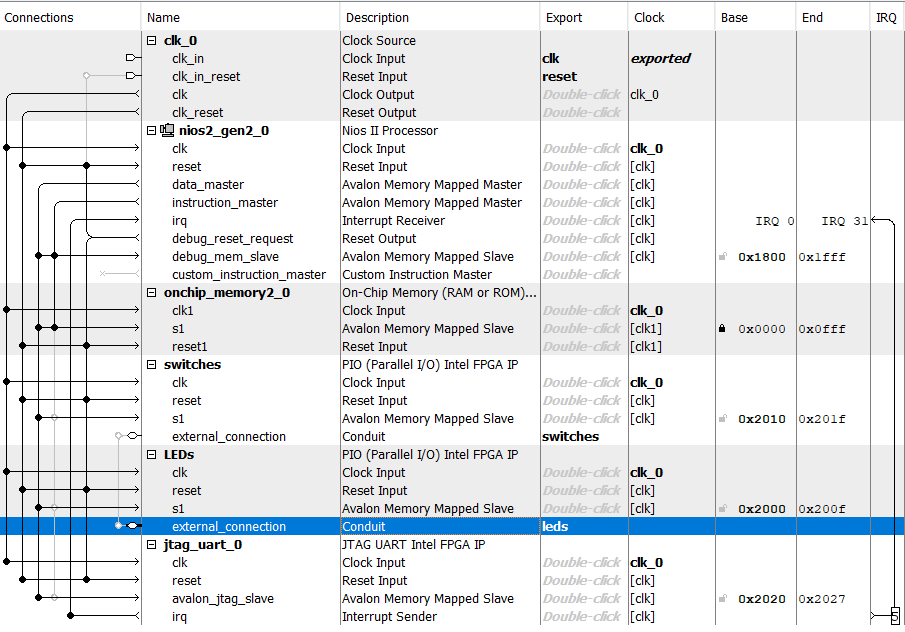
\includegraphics[scale=0.7]{figures/figure19.png}
   \end{center}
   \caption{The complete system.} 
	\label{fig:19}
\end{figure}
 
\item Having specified all components needed to implement the desired system,
it can now be generated.
Save the specified system; we used the name {\it nios\_system}. 
Then, select {\sf Generate > Generate HDL},
which leads to the window in Figure~\ref{fig:20}. 
Select {\sf None} for the option {\sf Simulation $>$ Create simulation model}, 
because in this tutorial we will not deal with the simulation of hardware. 
Click {\sf Generate} on the bottom of the window. 
When successfully completed, the generation process produces 
the message ``Generate Completed".

Exit the Platform Designer tool to return to the main Quartus Prime window.
\end{enumerate}

\begin{figure}[H]
   \begin{center}
      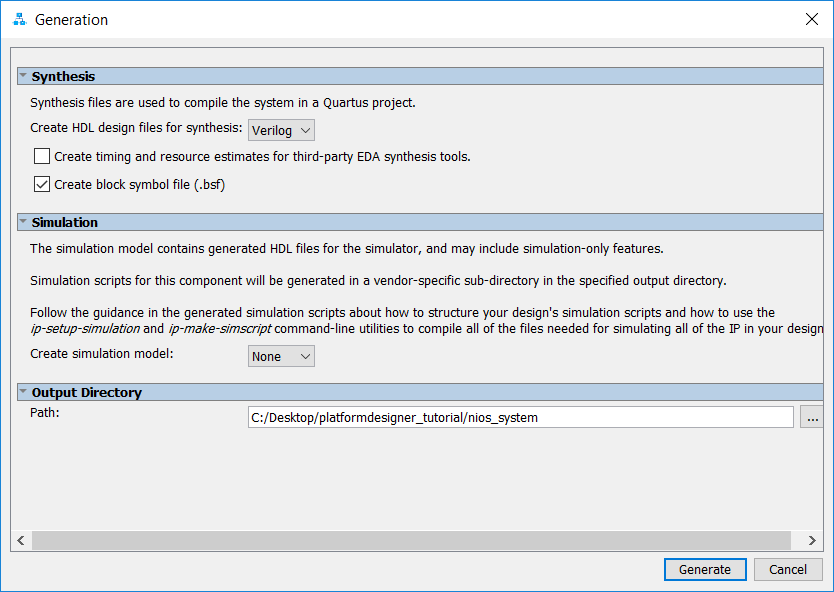
\includegraphics[scale=0.6]{figures/figure20.png}
   \end{center}
   \caption{Generation of the system.} 
	\label{fig:20}
\end{figure}

Changes to the designed system are easily made at any time by reopening the
Platform Designer tool. Any component in the System Contents
tab of the Platform Designer tool can be selected and edited or deleted, or a new component can be
added and the system regenerated.

\section{Integration of the Nios\textsuperscript{\textregistered} II System into a Quartus\textsuperscript{\textregistered} Prime Project}

To complete the hardware design, we have to perform the following:

\begin{itemize}
\item Instantiate the module generated by the Platform Designer tool into the Quartus Prime project
\item Assign the FPGA pins
\item Compile the designed circuit
\item Program and configure the FPGA device on the DE1-SoC board
\end{itemize}

\subsection{Instantiation of the Module Generated by the Platform Designer Tool}

The Platform Designer tool generates a Verilog module
% or VHDL module
that defines the desired Nios II system.
In our design, this module will have been generated in the {\it nios\_system.v} file,
which can be found in the directory 
{\it platformdesigner\_tutorial/nios\_system/synthesis} of the project.
The Platform Designer tool generates Verilog modules, which can then be used in designs
specified using either Verilog or VHDL languages.

Normally, the Nios II module generated by the Platform Designer tool is likely to be a part of a larger design. 
However, in the case of our simple example there is no other circuitry needed. 
All we need to do is instantiate the
Nios II system in our top-level Verilog or VHDL module, and connect inputs and outputs 
of the parallel I/O ports, as well as the clock and reset inputs, to the appropriate
pins on the FPGA device.

The Verilog code in the {\it nios\_system.v} file is quite large. Figure~\ref{fig:21} depicts
the portion of the code that defines the input and output ports for the
module {\it nios\_system}. The 8-bit vector that is the input to the parallel port 
{\it switches} is called {\it switches\_export}. 
The 8-bit output vector is called {\it leds\_export}. 
The clock and reset signals are called {\it clk\_clk} and {\it reset\_reset\_n}, respectively.
Note that the reset signal was added automatically by the Platform Designer tool;
it is called {\it reset\_reset\_n} because it is active low.
~\\

\begin{figure}[H]
   \begin{center}
      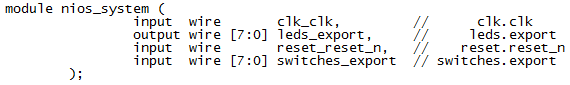
\includegraphics[scale=.6]{figures/figure21.png}
   \end{center}
   \caption{A part of the generated Verilog module.} 
	\label{fig:21}
\end{figure}

The {\it nios\_system} module has to be instantiated in a top-level module that has to be
named {\it lights}, because this is the name we specified
in Figure~\ref{fig:3} for the top-level design entity in our Quartus Prime project.
For the input and output ports of the {\it lights} module we have used the pin names
that are specified in the DE1-SoC User Manual: 
{\it CLOCK\_50} for the 50-MHz clock,  {\it KEY} for the pushbutton switches,
{\it SW} for the slider switches, and {\it LEDR} for the red LEDs.
Using these names simplifies the task of creating the needed pin assignments.

\newpage
\subsubsection{Instantiation in a Verilog Module}
Figure~\ref{fig:22} shows a top-level Verilog module that instantiates the Nios II system.
If using Verilog for the tutorial, 
type this code into a file called {\it lights.v}, or use the file provided with this tutorial.

\begin{figure}[H]
\begin{center}
\begin{lstlisting}[language=Verilog]

// Implements a simple Nios II system for the DE-series board.
// Inputs:   SW7-0 are parallel port inputs to the Nios II system
//           CLOCK_50 is the system clock
//           KEY0 is the active-low system reset
// Outputs:  LEDR7-0 are parallel port outputs from the Nios II system

module lights (CLOCK_50, SW, KEY, LEDR);
    input CLOCK_50;
    input [7:0] SW;
    input [0:0] KEY;
    output [7:0] LEDR;
// Instantiate the Nios II system module generated by the Platform Designer tool:
    nios_system NiosII (
        .clk_clk(CLOCK_50),
        .reset_reset_n(KEY),
        .switches_export(SW),
        .leds_export(LEDR));
endmodule

\end{lstlisting}
\end{center}
	\caption{Instantiating the Nios II system using Verilog code.}
	\label{fig:22}
\end{figure}

\newpage
\subsubsection{Instantiation in a VHDL Module}
Figure~\ref{fig:23} shows a top-level VHDL module that instantiates the Nios II system.
If using VHDL for the tutorial, 
type this code into a file called {\it lights.vhd}, or use the file provided with this tutorial.
  
\begin{figure}[H]
\begin{center}
\begin{lstlisting}[language=VHDL]
-- Implements a simple Nios II system for the DE-series board.
-- Inputs:    SW7-0 are parallel port inputs to the Nios II system
--            CLOCK_50 is the system clock
--            KEY0 is the active-low system reset
-- Outputs:   LEDR7-0 are parallel port outputs from the Nios II system

LIBRARY ieee;
USE ieee.std_logic_1164.ALL;
USE ieee.std_logic_unsigned.ALL;

ENTITY lights IS

PORT (
    CLOCK_50 : IN STD_LOGIC;
    KEY : IN STD_LOGIC_VECTOR (0 DOWNTO 0);
    SW : IN STD_LOGIC_VECTOR (7 DOWNTO 0);
    LEDR : OUT STD_LOGIC_VECTOR (7 DOWNTO 0)
    );
END lights;

ARCHITECTURE lights_rtl OF lights IS
    COMPONENT nios_system
    PORT (
        SIGNAL clk_clk: IN STD_LOGIC;
        SIGNAL reset_reset_n : IN STD_LOGIC;
        SIGNAL switches_export : IN STD_LOGIC_VECTOR (7 DOWNTO 0);
        SIGNAL leds_export : OUT STD_LOGIC_VECTOR (7 DOWNTO 0)
        );
    END COMPONENT;
BEGIN
NiosII : nios_system
    PORT MAP(
        clk_clk => CLOCK_50,
        reset_reset_n => KEY(0),
        switches_export => SW(7 DOWNTO 0),
        leds_export => LEDR(7 DOWNTO 0)
    );
END lights_rtl;
\end{lstlisting}
\end{center}
	\caption{Instantiating the Nios II system using VHDL code.}
	\label{fig:23}
\end{figure}


\section{Compiling the Quartus\textsuperscript{\textregistered} Prime Project}

Add the {\it lights.v/vhd} file to your Quartus Prime project.
Also, add the necessary pin assignments for the DE-series board to your project.
The procedure for making pin assignments is described in the tutorial 
{\it Quartus Prime Introduction Using Verilog/VHDL Designs}. Note that an easy way of
making the pin assignments when we use the same pin names as in the DE1-SoC 
User Manual is to import the assignments from a Quartus Prime Setting File with Pin Assignments. 
For example, the pin assignments for the DE1-SoC board are provided in the {\it DE1\_SoC.qsf} file, 
which can be found on Intel's FPGA University Program website. 

Since the system we are designing needs to operate at a 50-MHz clock
frequency, we can add the needed timing assignment in the Quartus Prime project.
The tutorial {\it Using TimeQuest Timing Analyzer} shows how this is done.
However, for our simple design, we can rely on the default timing assignment that the Quartus Prime
compiler assumes in the absence of a specific specification. The compiler assumes that the circuit
has to be able to operate at a clock frequency of 1 GHz, and will produce an implementation
that either meets this requirement or comes as close to it as possible.

Finally, before compiling the project, it is necessary to add the {\it nios\_system.qip}
file (IP Variation file) in the directory 
{\it platformdesigner\_tutorial/nios\_system/synthesis} to your Quartus Prime project.
Then, compile the project.
You may see some warning messages associated with
the Nios II system, such as some signals being unused or having wrong bit-lengths of vectors; 
these warnings can be ignored.

Note: Certain boards with MAX10 chips (eg. DE10-Lite) may require you to change the setting
{\sf Assignments > Device > Device and Pin Options > Configuration > Configuration Mode} to 
{\sf Single uncompressed image with Memory Initialization} in order to successfully compile.

\section{Using the \productNameMed{} to Download the Designed Circuit and Run an Application Program}

The designed circuit has to be downloaded into the FPGA device on a DE-series board. 
This can be done by using the Programmer Tool in the Quartus Prime software. 
However, we will use a simpler approach by using the \productNameMed{}, 
which provides a simple means for downloading
the circuit into the FPGA as well as running the application programs.

A parallel I/O interface generated by the Platform Designer tool is accessible by means of registers
in the interface. Depending on how the PIO is configured, there may be as many as
four registers. One of these registers is called the Data register. 
In a PIO configured as an input interface, the data read from the Data register is
the data currently present on the PIO input lines.
In a PIO configured as an output interface, the data written (by the Nios II processor)
into the Data register drives the PIO output lines.
If a PIO is configured as a bidirectional interface, then the PIO inputs and outputs
use the same physical lines. In this case there is a Data Direction register included,
which determines the direction of the input/output transfer.
In our unidirectional PIOs, it is only necessary to have the Data register.
The addresses assigned by the Platform Designer tool are 0x00002010 for the Data register in
the PIO called {\it switches} and 0x00002000 for the Data register in the PIO called {\it LEDs},
as indicated in Figure~\ref{fig:17}.

Our application task is very simple. A pattern selected by the current setting of slider 
switches has to be displayed on the LEDs. We will show how this can be done in both
Nios II assembly language and C programming language.

\subsection{A Nios II Assembly Language Program}
Figure 23 gives a Nios II assembly-language program that implements our task. 
The program loads the addresses of the Data registers in the two PIOs
into processor registers $r2$ and $r3$. It then has an infinite loop that merely
transfers the data from the input PIO, {\it switches}, to the output PIO, {\it leds}.

\begin{figure}[H]
\begin{center}
\begin{lstlisting}[style=defaultNiosStyle, xleftmargin=4cm]
.equ     switches, 0x00002010
.equ     leds, 0x00002000
.global  _start
_start:  movia   r2, switches
         movia   r3, leds
LOOP:    ldbio   r4, 0(r2)
         stbio   r4, 0(r3)
         br      LOOP
.end
\end{lstlisting}
\end{center}
	\caption{Assembly-language code to control the lights.}
	\label{fig:24}
\end{figure}

The directive ~~.global~~\_start ~~indicates
to the Assembler that the label  ~{\it \_start} is accessible outside the
assembled object file. This label is the default label we use to indicate to
the Linker program the beginning of the application program.

For a detailed explanation of the Nios II assembly language instructions see
the tutorial {\it Introduction to the Intel Nios II Soft Processor},
which is available on Intel's FPGA University Program website.

Enter this code into a file {\it lights.s}, or use the file provided with this tutorial,
and place the file into a working directory. We placed the file into the directory 
{\it platformdesigner\_tutorial$\backslash$app\_software}.

\subsection{A C-Language Program}
An application program written in the C language can be handled in the same way as 
the assembly-language program. A C program that implements our simple task is 
given in Figure 24. Enter this code into a file called {\it lights.c},
or use the file provided with this tutorial, and place the file into a working directory. 
\\
\begin{figure}[H]
\begin{center}
\begin{lstlisting}[language=C]
#define switches (volatile char *) 0x0002010
#define leds (char *) 0x0002000
void main()
{         while (1)
          *leds = *switches;
}
\end{lstlisting}
\end{center}
	\caption{C-language code to control the lights.}
	\label{fig:25}
\end{figure}

\subsection{Using the \productNameMed{}}
The FPGA University Program provides the {\it monitor} software, called {\it \productNameMed{}}, 
for use with the DE-series boards. This software provides a simple means for compiling, assembling
and downloading of programs onto a DE-series board.
It also makes it possible for the user to perform debugging tasks.
A description of this software is available in the {\it \productNameMed{}} tutorial.
We should also note that other Nios II development systems are provided by Intel,
for use in commercial development.
Although we will use the \productNameMed{} in this tutorial, the other Nios II tools
available from Intel could alternatively be used with our designed hardware system.

Open the \productNameMed{}, which leads to the window in Figure~\ref{fig:26}.
~\\

\begin{figure}[H]
   \begin{center}
      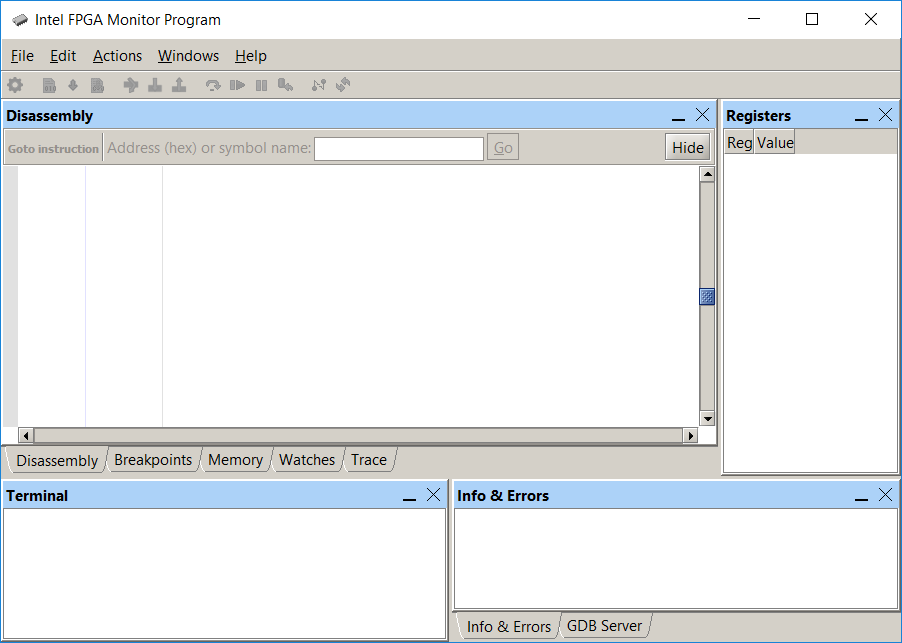
\includegraphics[scale=0.7]{figures/figure26.png}
   \end{center}
   \caption{The \productNameMed{} main window.} 
	\label{fig:26}
\end{figure}

\newpage
\noindent 
The monitor program needs to know the characteristics
of the designed Nios II system, which are given in the file {\it nios\_system.qsys}.  
Click the {\sf File > New Project} menu item to display the New Project Wizard window, shown in
Figure~\ref{fig:27}, and perform the following steps:

\begin {enumerate}
  \item Enter the {\it platformdesigner\_tutorial$\backslash$app\_software} directory as the Project directory by
typing it directly into the Project directory field, or by browsing to it using the {\sf Browse...} button.
\item Enter {\it lights\_example} (or some other name) as the Project name
\item Select {\sf Nios II} as the Architecture and click {\sf Next}, 
leading to Figure~\ref{fig:28}.
~\\
%~\\

\begin{figure}[H]
   \begin{center}
      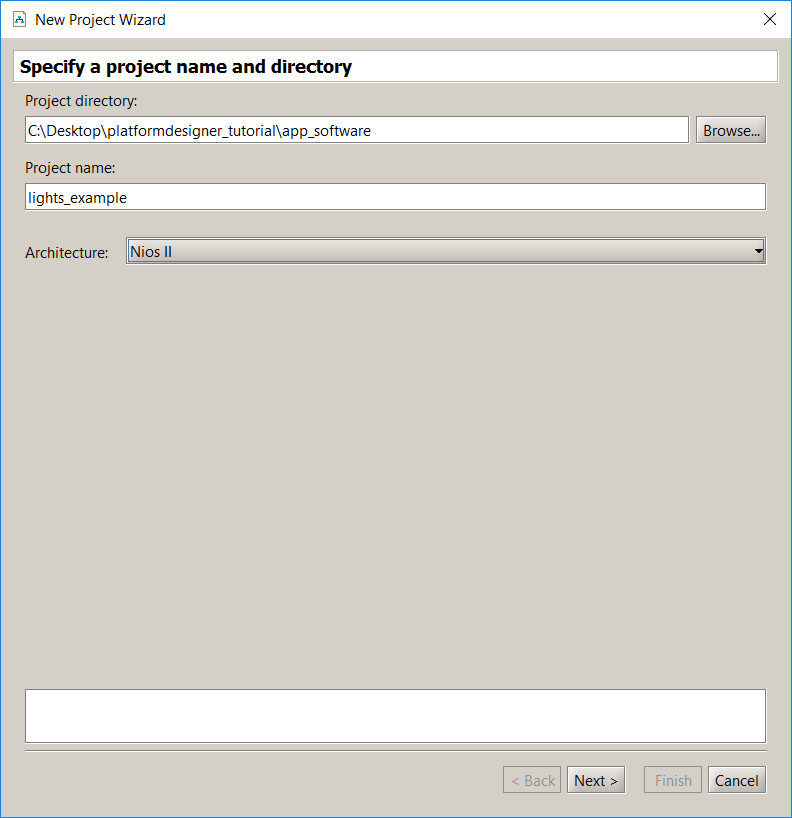
\includegraphics[scale=0.6]{figures/figure27.png}
   \end{center}
   \caption{Specify the project directory and name.} 
	\label{fig:27}
\end{figure}

\begin{figure}[H]
   \begin{center}
      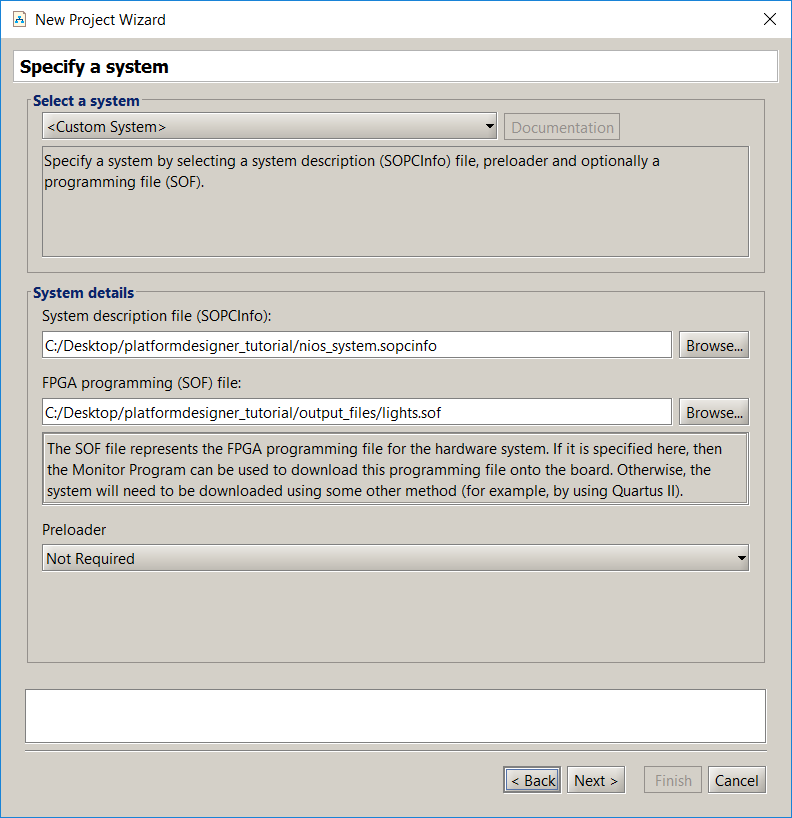
\includegraphics[scale=0.6]{figures/figure28.png}
   \end{center}
   \caption{The System Specification window.} 
	\label{fig:28}
\end{figure}

  \item From the {\sf Select a System} drop-down box select {\sf Custom System},
which specifies that you wish to use the hardware that you designed.
~\\

Click {\sf Browse...} beside the {\sf System description} field to display a file selection window 
and choose the {\it nios\_system.sopcinfo} file. Note that this file is in the design 
directory {\it platformdesigner\_tutorial}. 
~\\

Select the {\it lights.sof} file in the {\sf FPGA programming (SOF) file} field, 
which provides the information needed to download the designed system into the FPGA device on the DE-series board. Note that this file is in the design directory {\it platformdesigner\_tutorial/output\_files}. 
\\

Finally, for the {\sf Preloader} field, select {\it Not Required}.
Click {\sf Next}, which leads to the window in Figure~\ref{fig:29}.

\begin{figure}[H]
   \begin{center}
      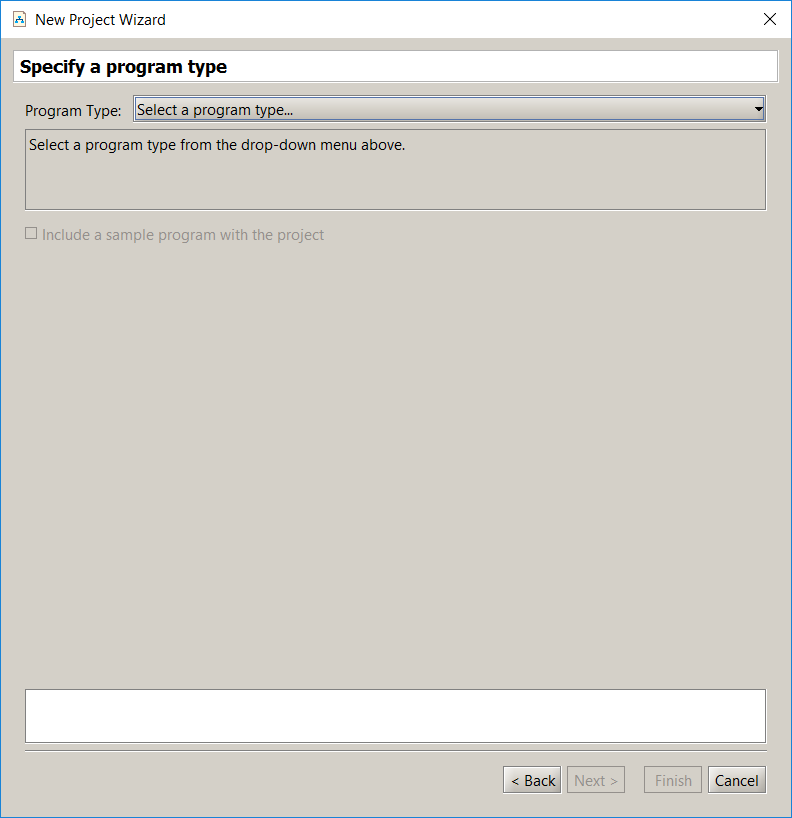
\includegraphics[scale=0.7]{figures/figure29.png}
   \end{center}
   \caption{Specification of the program type.} 
	\label{fig:29}
\end{figure}

	\item If you wish to use a Nios II assembly-language application program, 
select {\sf Assembly Program} as the program type from the drop-down menu. 
If you wish to use a C-language program, select {\sf C Program}.
Click {\sf Next}, leading to Figure~\ref{fig:30}. 
	\item Click {\sf Add...} to display a file selection window and choose the {\it lights.s} file,
or {\it lights.c} for a C program,
and click {\sf Select}. For this tutorial, we have chosen to use the assembly program.
We placed the application-software files in the directory {\it platformdesigner\_tutorial$\backslash$app\_software}.
Upon returning to the window in Figure~\ref{fig:30}, click {\sf Next}.

\begin{figure}[H]
   \begin{center}
      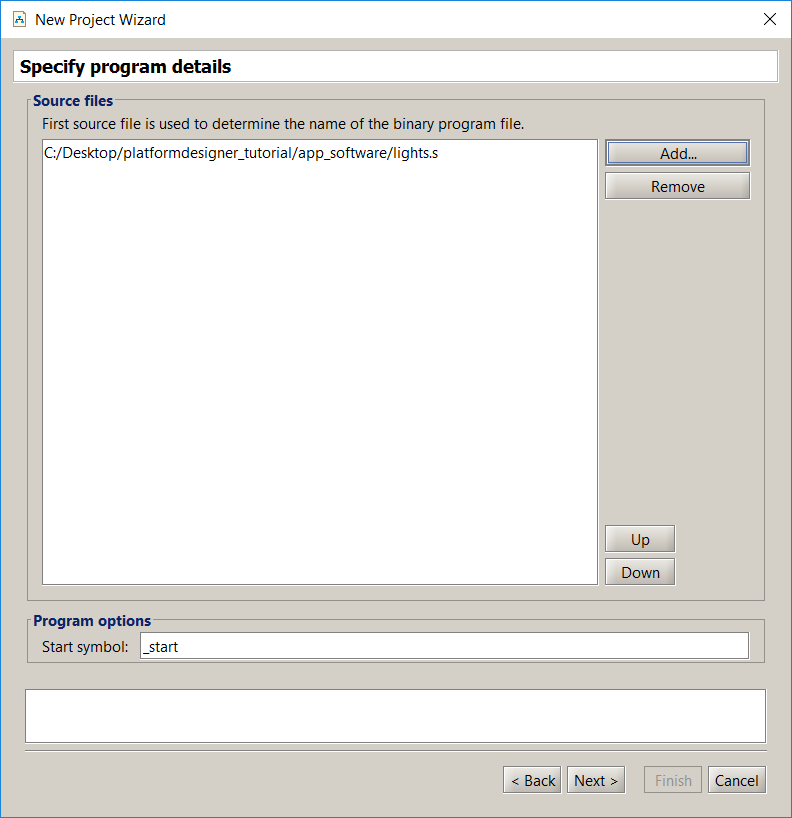
\includegraphics[scale=0.7]{figures/figure30.png}
   \end{center}
   \caption{Specify the application program to use.} 
	\label{fig:30}
\end{figure}
~\\

	\item In the window in Figure~\ref{fig:31}, ensure that the {\sf Host Connection} is set corresponding to your target board. Here, we are using the DE1-SoC board, and so have set it to {\it DE-SoC}, 
the {\sf Processor} is set to {\it nios2\_qsys\_0} and the {\sf Terminal Device} is set to {\it jtag\_uart\_0}. 
Click {\sf Next}.
~\\

\begin{figure}[H]
   \begin{center}
      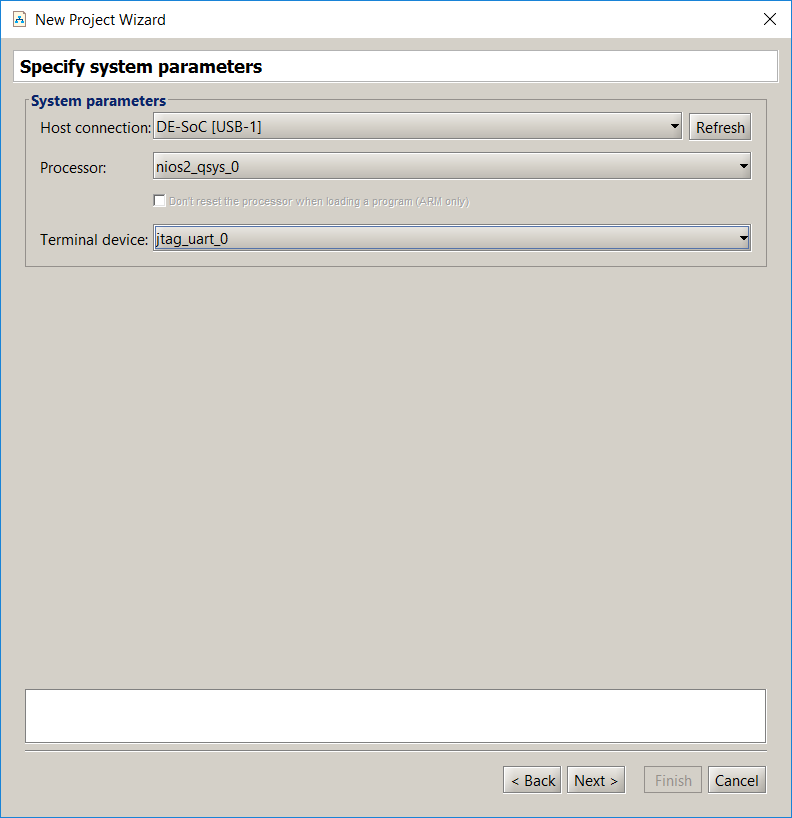
\includegraphics[scale=0.7]{figures/figure31.png}
   \end{center}
   \caption{Specify the system parameters.} 
	\label{fig:31}
\end{figure}

	\item The Monitor Program also needs to know where to load the application program. 
In our case, this is the memory block in the FPGA device. The name assigned to this memory
is {\it onchip\_memory}.
Since there is no other memory in our design, the Monitor Program will select this memory by default,
as shown in Figure~\ref{fig:32}. 
~\\

Having provided the necessary information, click {\sf Finish} to confirm the system configuration.
When a pop-up box asks you if you want to have your system downloaded onto the DE-series board click {\sf Yes}.

\begin{figure}[H]
   \begin{center}
      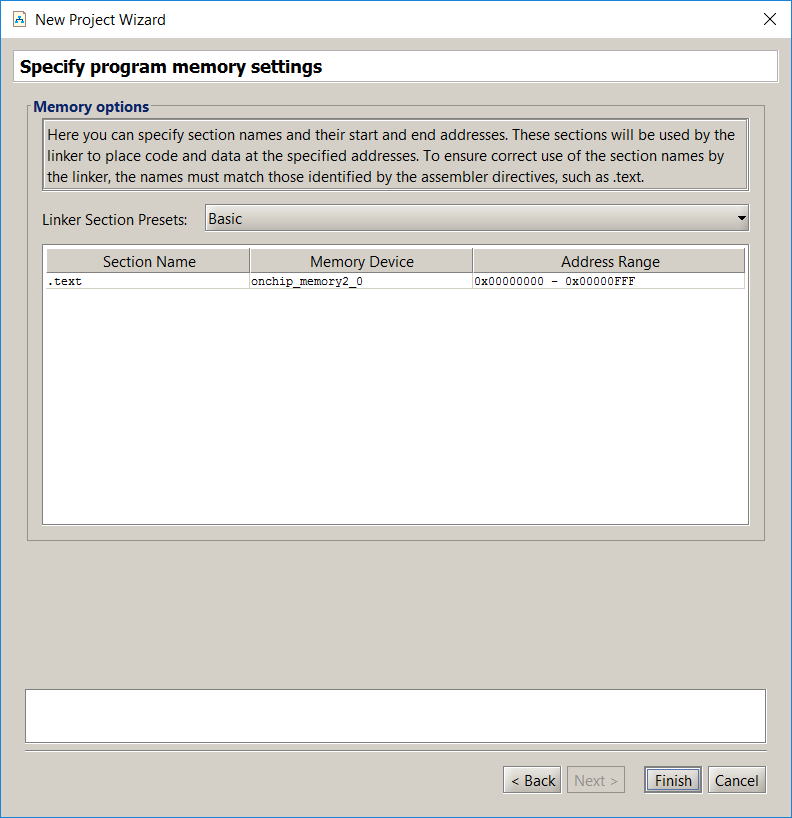
\includegraphics[scale=0.7]{figures/figure32.png}
   \end{center}
   \caption{Specify where the program will be loaded in the memory.} 
	\label{fig:32}
\end{figure}

	\item Now, in the monitor window in Figure~\ref{fig:26} select {\sf Actions $>$ Compile \& Load}
to assemble and download your program.

\item The downloaded program is shown in Figure~\ref{fig:33}. 
Run the program and verify the correctness of the designed system by setting the slider switches to
a few different patterns.

\end{enumerate}

\begin{figure}[H]
   \begin{center}
      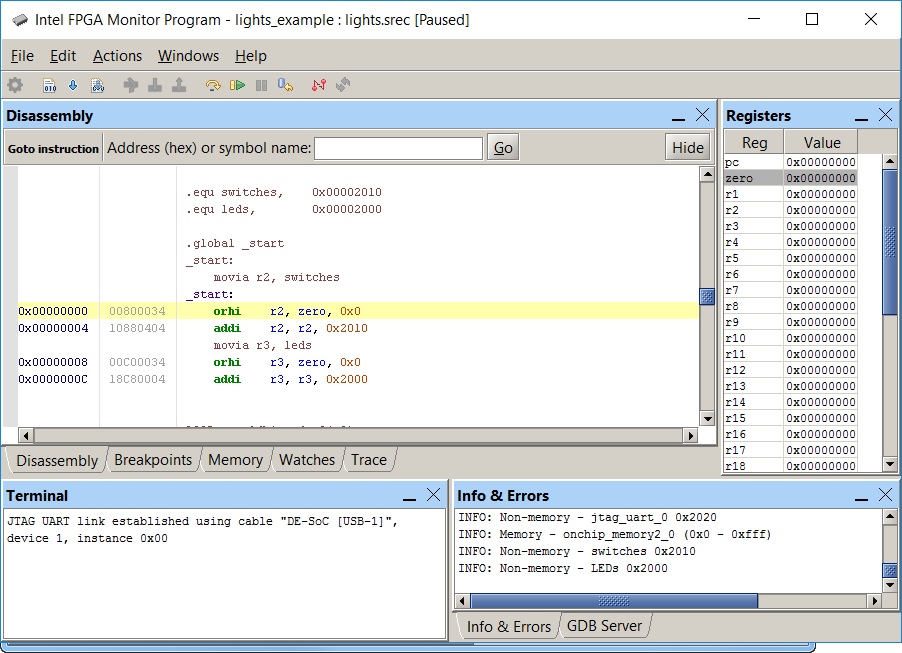
\includegraphics[scale=0.6]{figures/figure33.png}
   \end{center}
   \caption{Display of the downloaded program.} 
	\label{fig:33}
\end{figure}

% Copyright and Trademark

%\newcommand{\datePublished}{Mar 2022}

\newcommand{\versnum}{21.1} %version number quartus/AMP
\newcommand{\quartusname}{Quartus\textsuperscript{\textregistered} Prime}	
\newcommand{\textBar}{For \quartusname{} \versnum{}}
\newcommand{\thisyear}{2022 } %for copyright
\newcommand{\company}{FPGAcademy.org}
\newcommand{\longteamname}{FPGAcademy.org}
\newcommand{\teamname}{FPGAcademy}
\newcommand{\website}{FPGAcademy.org}

\newcommand{\productAcronym}{AMP}
\newcommand{\productNameShort}{Monitor Program}

\newcommand{\productNameMedTM}{Monitor Program}
\newcommand{\productNameMed}{Monitor Program}

%\newcommand{\headerLogoFilePath}[1]{#1/FPGAcademy.png}



%%%%%%%%%%%%%%%%%%%%%%%%%%%%%%%%%%%%%%%%
%%% FPGAcademy Copyright Information %%%
%%%%%%%%%%%%%%%%%%%%%%%%%%%%%%%%%%%%%%%%

%Always put the copyright on a new page (clear page), with some vertical space from top
\clearpage
\vspace{1in}

\noindent

Copyright {\copyright} FPGAcademy.org. All rights reserved. FPGAcademy and the FPGAcademy logo are trademarks of  FPGAcademy.org.  This document is being provided on an ``as-is'' basis and as an accommodation and therefore all warranties, representations or guarantees of any kind (whether express, implied or statutory) including, without limitation, warranties of merchantability, non-infringement, or fitness for a particular purpose, are specifically disclaimed.

%FPGAcademy assumes no responsibility or liability arising out of the application or use of any information,  product,  or  service  described  herein  except  as  expressly  agreed  to  in  writing  by  FPGAcademy.



**Other names and brands may be claimed as the property of others.





\end{document}
